\documentclass[11pt,a4paper]{article}

% ---------------------------------------------------------------- packages
\usepackage[utf8]{inputenc}
\usepackage[T1]{fontenc}
\usepackage{lmodern}
\usepackage[margin=2.2cm]{geometry}
\usepackage{graphicx}
\usepackage{booktabs}
\usepackage{tabularx}
\usepackage{array}
\usepackage{amsmath}
\usepackage{xcolor}
\usepackage{float}
\usepackage{caption}
\usepackage{subcaption}
\usepackage{enumitem}
\usepackage{fancyhdr}
\usepackage{titlesec}
\usepackage[framemethod=default]{mdframed}
\usepackage{textcomp}
\usepackage{gensymb}
\usepackage[hidelinks]{hyperref}

\graphicspath{{../outputs/figures/}}
\definecolor{ucunavy}{HTML}{0B3D91}
\definecolor{ucured}{HTML}{D7014D}
\definecolor{tint}{HTML}{EEF3FA}
\definecolor{todo}{HTML}{FFF3CD}

\titleformat{\section}{\Large\bfseries\color{ucunavy}}{\thesection}{0.6em}{}
\titleformat{\subsection}{\large\bfseries\color{ucunavy}}{\thesubsection}{0.6em}{}
\titleformat{\subsubsection}{\normalsize\bfseries\color{ucured}}{\thesubsubsection}{0.6em}{}

\pagestyle{fancy}
\fancyhf{}
\lhead{\small CSC3119 AI Deployment \& Scalability}
\rhead{\small Assignment 4 -- AirQo PM2.5 Prediction}
\cfoot{\small\thepage}
\setlength{\headheight}{14pt}
\setlength{\parskip}{0.45em}
\setlength{\parindent}{0pt}
\setlength{\emergencystretch}{3em}
\sloppy
\setlist{itemsep=0.15em,topsep=0.3em}
\captionsetup{font=small,labelfont={bf,color=ucunavy}}

\newcommand{\ugm}{\,\textmu g/m\textsuperscript{3}}
\newmdenv[backgroundcolor=tint,linewidth=0pt,innerleftmargin=10pt,innerrightmargin=10pt,innertopmargin=8pt,innerbottommargin=8pt]{keybox}
\newmdenv[backgroundcolor=todo,linewidth=0pt,innerleftmargin=10pt,innerrightmargin=10pt,innertopmargin=8pt,innerbottommargin=8pt]{todobox}
\newcolumntype{L}[1]{>{\raggedright\arraybackslash}p{#1}}
\newcolumntype{Y}{>{\raggedright\arraybackslash}X}

% ---------------------------------------------------------------- title
\title{\vspace{-1.2cm}\textcolor{ucunavy}{\textbf{Predicting PM2.5 Air Quality Concentrations\\from AirQo Sensor Data}}\\[0.4em]
\large An end-to-end pipeline: data preparation, exploratory analysis, machine learning,\\ forecasting, monitoring with Evidently AI and deployment on RunPod}
\author{Mirembe Peace Mercy (M24B23/005 / B27499)\\
Norah Angel Nakaye (M24B23/008 / B27502)\\[0.3em]
\small Uganda Christian University --- CSC3119 AI Deployment \& Scalability, Assignment 4}
\date{4 October 2026}

\begin{document}
\maketitle
\thispagestyle{empty}

\begin{abstract}
\noindent
Fine particulate matter (PM2.5) is the air pollutant with the largest health burden in Kampala, where the annual mean concentration is about eight times the WHO guideline. We build a complete, reproducible pipeline that predicts hourly PM2.5 from AirQo low-cost sensor data (14{,}600 hourly records, 149 sensors). An audit showed that the file labelled January--July 2026 contains only three short observation windows (1--3 January, 1--2 April and 1--3 June). We resample every sensor onto a complete hourly grid, treat offline hours as missing rather than absent, interpolate only short gaps, and impute missing temperature and humidity spatially. Exploratory analysis of five Kampala sensors reveals a strongly right-skewed distribution, a clear morning and evening peak, much higher pollution in the January dry season, a negative association with temperature and a positive one with humidity. Five tuned models (Ridge, K-nearest neighbours, support vector regression, random forest, XGBoost) and a stacking ensemble are trained on the Z-score of PM2.5 with blocked, leave-days-out cross-validation and evaluated on the last 24 observed hours. XGBoost is the best model (RMSE 20.0\ugm, MAE 12.3\ugm, $R^2=0.22$, 71\% AQI-category accuracy), and all models beat the baselines. The saved model produces daily forecasts for 1--16 August 2026 and hourly forecasts for 1 August 2026, which are inverse-transformed to \ugm{} and visualised against AQI bands, including a shapefile-based map of at-risk sensors. Evidently AI shows seasonal drift in temperature, humidity and the target and a 36\% rise in RMSE on unseen data. The pipeline is packaged to run headless on a RunPod GPU pod.
\end{abstract}

\tableofcontents
\newpage

% =================================================================
\section{Introduction}
AirQo, an air-quality initiative at Makerere University, designs and manufactures low-cost monitors for African cities and runs a network of more than 350 devices that measure PM2.5, PM10 and NO\textsubscript{2}. PM2.5 --- particles smaller than 2.5\,\textmu m --- bypasses the body's upper-airway defences, reaches the alveoli and can enter the bloodstream; long-term exposure is linked to respiratory and cardiovascular disease, stroke and premature death. A four-year reference-grade study in Kampala (2018--2021) found an annual mean of 39\ugm{}, about eight times the WHO guideline of 5\ugm{}, and attributed about 7{,}257 deaths to long-term PM2.5 exposure.

Forecasting PM2.5 turns a sparse, sensor-limited picture into forward-looking situational awareness for the health sector (early warning of admissions), the National Environment Management Authority (enforcement and siting), the Ministry of Energy (clean-cooking programmes) and the Ministry of Works and Transport (traffic and fleet policy).

\textbf{Objective.} Build a deployable pipeline that predicts PM2.5 concentration (as a Z-score) from AirQo sensor data --- from raw data to a trained, evaluated, monitored and cloud-deployed model --- and use it to forecast PM2.5 for August 2026.

Throughout, we use the AQI categories in Table~\ref{tab:aqi}.

\begin{table}[H]
\centering\small
\caption{PM2.5 AQI categories used in all visualisations and evaluations.}
\label{tab:aqi}
\begin{tabular}{lll}
\toprule
PM2.5 (\ugm) & Category & Colour \\
\midrule
0 -- 9 & Good & green \\
9.101 -- 35.49 & Moderate & yellow \\
35.491 -- 55.49 & Unhealthy for Sensitive Groups (USG) & orange \\
55.491 -- 125.49 & Unhealthy & red \\
125.491 -- 225.49 & Very Unhealthy & purple \\
$>$ 225.49 & Hazardous & maroon \\
\bottomrule
\end{tabular}
\end{table}

% =================================================================
\section{Methodology overview}
Figure~\ref{fig:pipeline} shows the pipeline. Every stage writes its outputs to disk and is timed by a logger, so a single run produces the evidence needed for deployment. Optional or fragile steps (Evidently, GPU detection, map plotting) are wrapped in \texttt{try/except} so that the pipeline never crashes.

\begin{figure}[H]
\centering
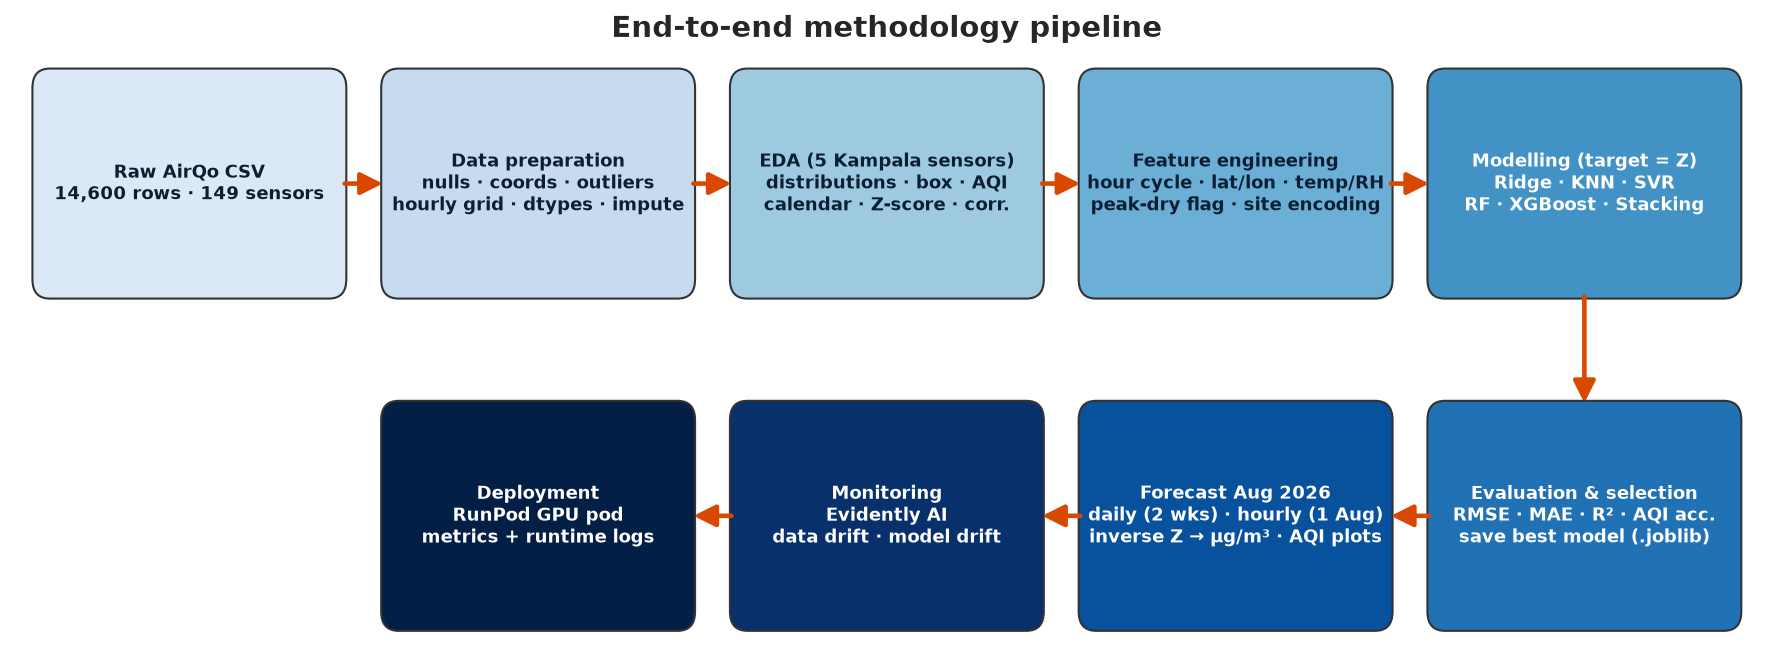
\includegraphics[width=\textwidth]{00_pipeline_flowchart.png}
\caption{End-to-end methodology pipeline.}
\label{fig:pipeline}
\end{figure}

The code lives in a single notebook (\texttt{AirQo\_PM25\_Pipeline.ipynb}, generated from \texttt{notebook\_src/airqo\_pm25\_pipeline.py}). All paths are relative, so the same notebook runs locally and on RunPod. The random seed is fixed at 42.

% =================================================================
\section{Data preparation}
\subsection{Dataset and audit}
The dataset has 14{,}600 hourly rows from 149 sensors at 145 named sites. Fields include site and device identifiers, network (AirQo or AirGradient hardware), coordinates, temperature, relative humidity and calibrated PM2.5 and PM10. Table~\ref{tab:audit} summarises the audit.

\begin{table}[H]
\centering\small
\caption{Raw data audit. Per the brief, a value of 0 is a null for these fields.}
\label{tab:audit}
\begin{tabular}{lrrr}
\toprule
Field & Empty & Zero & \% null (empty + zero) \\
\midrule
latitude & 1 & 3{,}085 & 21.1 \\
longitude & 0 & 3{,}067 & 21.0 \\
temperature & 54 & 4{,}066 & 28.2 \\
humidity & 206 & 4{,}159 & 29.9 \\
pm2\_5\_calibrated\_value & 325 & 0 & 2.2 \\
pm10\_calibrated\_value & 427 & 3 & 2.9 \\
site\_id & 7{,}508 & -- & 51.4 \\
\bottomrule
\end{tabular}
\end{table}

Four findings shaped every later decision:
\begin{enumerate}
\item \textbf{Three short windows, not a continuous series.} The file contains only 147 distinct timestamps: 1--3 January, 1--2 April and 1--3 June 2026. Each sensor has between 20 and 147 records.
\item \textbf{Zeros are nulls.} About 28--30\% of temperature and humidity values and 21\% of coordinates are zero; Kampala is never at 0\degree C and no sensor is at 0\degree N 0\degree E.
\item \textbf{Uninformative fields.} \texttt{frequency} is constant (\texttt{hourly}); \texttt{site\_id} is 51\% empty and duplicates \texttt{site\_name}.
\item \textbf{Implausible values and GPS jitter.} PM2.5 reaches 998\ugm{} (sensor saturation). Fixed sensors report up to 119 distinct GPS positions, and six devices never report a valid fix.
\end{enumerate}

\subsection{Literature guiding the cleaning}
Junninen et al.\ \cite{junninen2004} compared imputation methods on air-quality data and found that simple linear interpolation is the most accurate for short gaps of a few hours, while longer gaps require multivariate (spatial or regression) methods and should not be filled with synthetic values without care. The AirQo team's characterisation study \cite{okure2022} describes device outages caused by power and 2G connectivity and works with hourly aggregates and completeness thresholds rather than filling long outages. The \texttt{*\_calibrated\_value} fields come from AirQo's machine-learning field calibration \cite{adong2022}, which already uses temperature and humidity, so we model the calibrated values directly. Barkjohn et al.\ \cite{barkjohn2021} remove physically implausible low-cost sensor readings before modelling. Table~\ref{tab:cleaning} lists the resulting policy.

\begin{table}[H]
\centering\small
\caption{Data-cleaning policy and justification.}
\label{tab:cleaning}
\begin{tabularx}{\textwidth}{L{4.3cm}L{4.4cm}Y}
\toprule
Situation & Action & Justification \\
\midrule
0 or empty in temperature, humidity, PM2.5, PM10, lat, lon & Set to NaN; a coordinate pair is valid only if both parts are & Defined as null in the brief \\
Mixed types, UTC strings & Datetime $\rightarrow$ Africa/Kampala local time; numerics $\rightarrow$ float64; identifiers $\rightarrow$ string & Consistent types; diurnal patterns follow local time \\
PM2.5 $>$ 500\ugm{} (3 rows) & NaN, logged & Beyond the low-cost sensor range \cite{barkjohn2021} \\
Per-sensor 1.5$\times$IQR outliers (650 rows; 222 beyond 3$\times$IQR) & Flagged and kept & Real rush-hour and inversion episodes \\
PM2.5 $>$ PM10 (2{,}994 rows) & Flagged and kept & Separate calibrations; PM10 is not a predictor \\
Gap $\le$ 3 h & Linear interpolation in time, per sensor, inside the window only & Accurate for short gaps \cite{junninen2004} \\
Gap $>$ 3 h (device offline) & Left NaN, \texttt{is\_observed} = 0, not used as targets & No fabricated labels \cite{okure2022} \\
Missing temperature/humidity at an observed hour & IDW of the 3 nearest sensors ($\le$ 50 km) at the same hour $\rightarrow$ sensor hour-of-day median $\rightarrow$ network median & Weather is spatially smooth \cite{junninen2004} \\
Missing or jittery coordinates & Per-device median; documented gazetteer for 6 devices & Fixed installations \\
\bottomrule
\end{tabularx}
\end{table}

\subsection{Hourly resampling and imputation}
Every sensor was placed on a complete hourly index from 1 January 00:00 to 31 July 23:00 (local time): 149 sensors $\times$ 5{,}088 hours $=$ 758{,}112 rows. Offline hours appear as explicit rows with missing values, so outages are visible rather than silently absent. Only 14{,}272 rows (1.88\%) carry a valid PM2.5 value before interpolation (Figure~\ref{fig:completeness}).

Short-gap interpolation filled 1{,}976 PM2.5, 2{,}026 PM10, 1{,}731 temperature and 1{,}773 humidity values. At observed hours, inverse-distance weighting
\begin{equation}
\hat{T}_{s,t} = \frac{\sum_{k=1}^{3} w_k T_{k,t}}{\sum_{k=1}^{3} w_k}, \qquad w_k = \frac{1}{\max(d_{s,k},\,0.5\text{ km})^2}
\end{equation}
filled 3{,}661 temperature and 3{,}807 humidity values from neighbouring sensors, and the sensor hour-of-day median filled a further 460 and 508. Every imputed row is flagged (\texttt{met\_imputed}). The cleaned grid is saved as \texttt{data/processed/hourly\_grid\_clean.parquet}.

\begin{figure}[H]
\centering
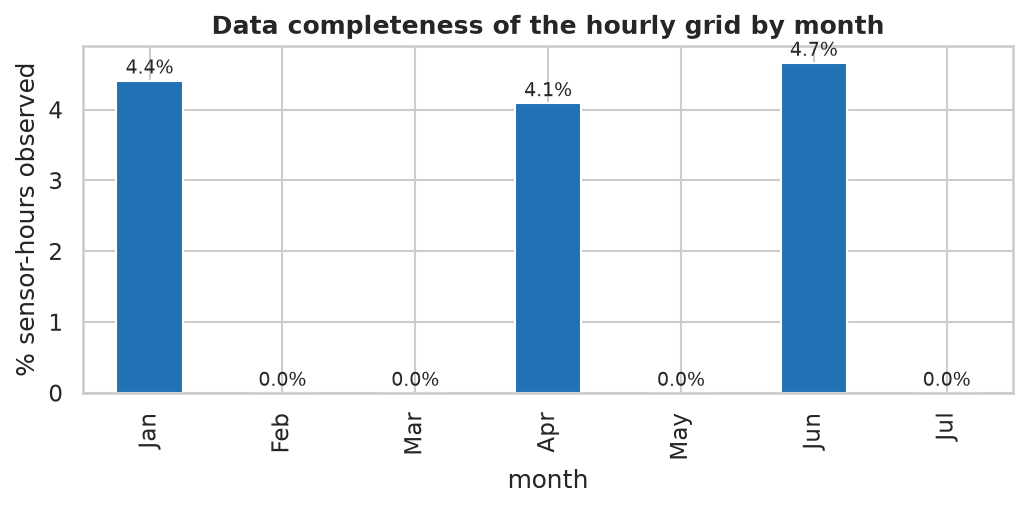
\includegraphics[width=0.6\textwidth]{02_completeness_by_month.png}
\caption{Share of sensor-hours with a valid PM2.5 value, by month.}
\label{fig:completeness}
\end{figure}

\subsection{Feature selection}
\begin{table}[H]
\centering\small
\caption{Feature selection.}
\label{tab:features}
\begin{tabularx}{\textwidth}{L{4.2cm}L{1.2cm}Y}
\toprule
Field & Used? & Reasoning \\
\midrule
PM2.5 & Target & Global Z-score of calibrated PM2.5 \\
Temperature, humidity & Yes & Boundary-layer height and hygroscopic growth drive PM2.5 \\
Hour of day ($\sin$, $\cos$) & Yes & Diurnal cycle of traffic, cooking and night-time inversions; cyclic encoding keeps 23:00 next to 00:00 \\
Peak dry season (Dec--Feb) & Yes & Daily means 44--55\ugm{} in January vs.\ 21--28\ugm{} in April and June (Table~\ref{tab:daily}); August is coded 0 \\
Latitude, longitude & Yes & Spatial pattern: city centre vs.\ suburbs vs.\ towns \\
Device level & Yes & Smoothed, season-adjusted target encoding (training data only) \\
Network & Yes & AirQo vs.\ AirGradient hardware offsets \\
PM10 & No & Same sensor and time $\Rightarrow$ leakage; unavailable at forecast time; dust-driven \\
site\_name, site\_id, frequency & No & Identifiers or constant \\
Day of week & No & Only Monday--Friday are observed \\
\bottomrule
\end{tabularx}
\end{table}

The device level of sensor $s$ is the shrunk mean of its deviation from the network mean of the same observation window,
\begin{equation}
e_s = \frac{n_s\,\bar{\delta}_s}{n_s + m}, \qquad \delta_{s,t} = z_{s,t} - \bar{z}_{\text{window}(t)}, \quad m = 10 ,
\end{equation}
which separates each site's typical level from the season and shrinks sensors with few observations towards zero.

\begin{table}[H]
\centering\small
\caption{Network-wide daily statistics after cleaning (PM2.5 in \ugm), showing the January peak.}
\label{tab:daily}
\begin{tabular}{lrrrrr}
\toprule
Date & Mean PM2.5 & Median PM2.5 & Mean temp.\ (\degree C) & Mean RH (\%) & Rows \\
\midrule
1 Jan 2026 & 54.7 & 55.8 & 24.4 & 71.3 & 2{,}352 \\
2 Jan 2026 & 43.6 & 37.2 & 24.9 & 75.1 & 2{,}722 \\
1 Apr 2026 & 20.7 & 14.4 & 24.2 & 79.7 & 2{,}253 \\
2 Apr 2026 & 26.6 & 17.4 & 24.4 & 80.0 & 2{,}677 \\
1 Jun 2026 & 24.5 & 16.9 & 24.3 & 78.9 & 2{,}199 \\
2 Jun 2026 & 23.7 & 16.3 & 23.1 & 81.9 & 2{,}520 \\
\bottomrule
\end{tabular}

\smallskip
{\footnotesize Partial days (3 Jan, 3 Apr, 3 Jun; fewer than 620 rows each) are omitted; full table in Section 2.9 of the notebook.}
\end{table}

% =================================================================
\section{Exploratory data analysis}
EDA uses five Kampala sensors that have their own temperature and humidity probes and the most observations: Nansana east ward (Wakiso), Nakasero II, Lower Nsooba (Kawempe), Civic Centre (Kampala Central) and Salama Road (762 observed hours in total).

\subsection{Distributions and outliers}
PM2.5 is strongly right-skewed (skewness 2.09; mean 45.7\ugm{}, median 31.7\ugm{}, maximum 291\ugm{}), with many moderate hours and a few very high spikes (Figure~\ref{fig:dist}). Box plots per sensor (Figure~\ref{fig:box}) show that Salama Road (median 53.9\ugm) and Civic Centre have the highest levels and longest tails. Outliers beyond 1.5$\times$IQR (Civic Centre 17, Nansana 11, Salama Road 5) coincide with rush hours and night-time inversions, so they were flagged and kept: removing them would teach the model that unhealthy hours never happen.

\begin{figure}[H]
\centering
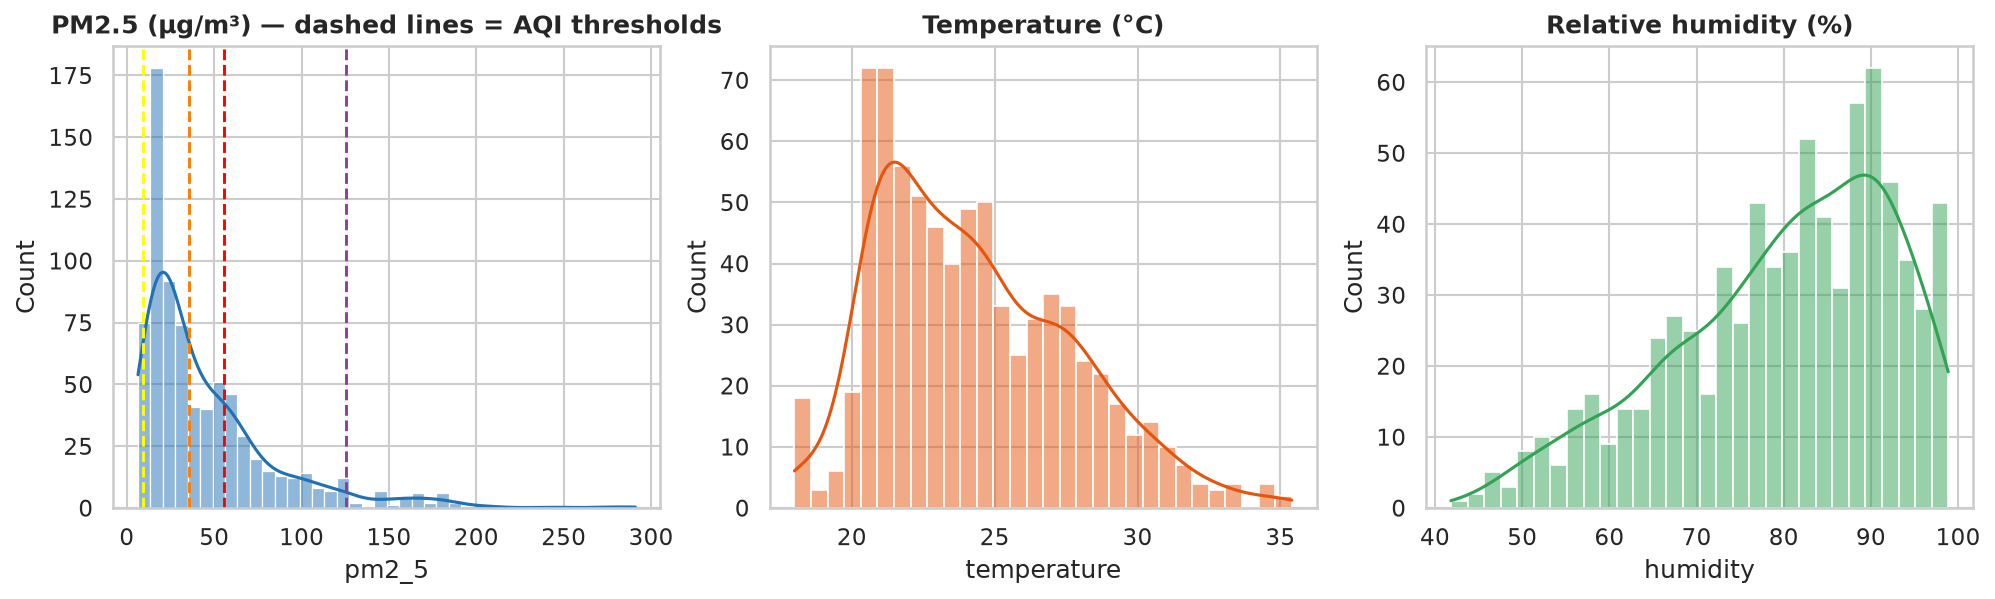
\includegraphics[width=\textwidth]{03_distributions.png}
\caption{Distributions of PM2.5 (dashed lines: AQI thresholds), temperature and humidity for the five EDA sensors.}
\label{fig:dist}
\end{figure}

\begin{figure}[H]
\centering
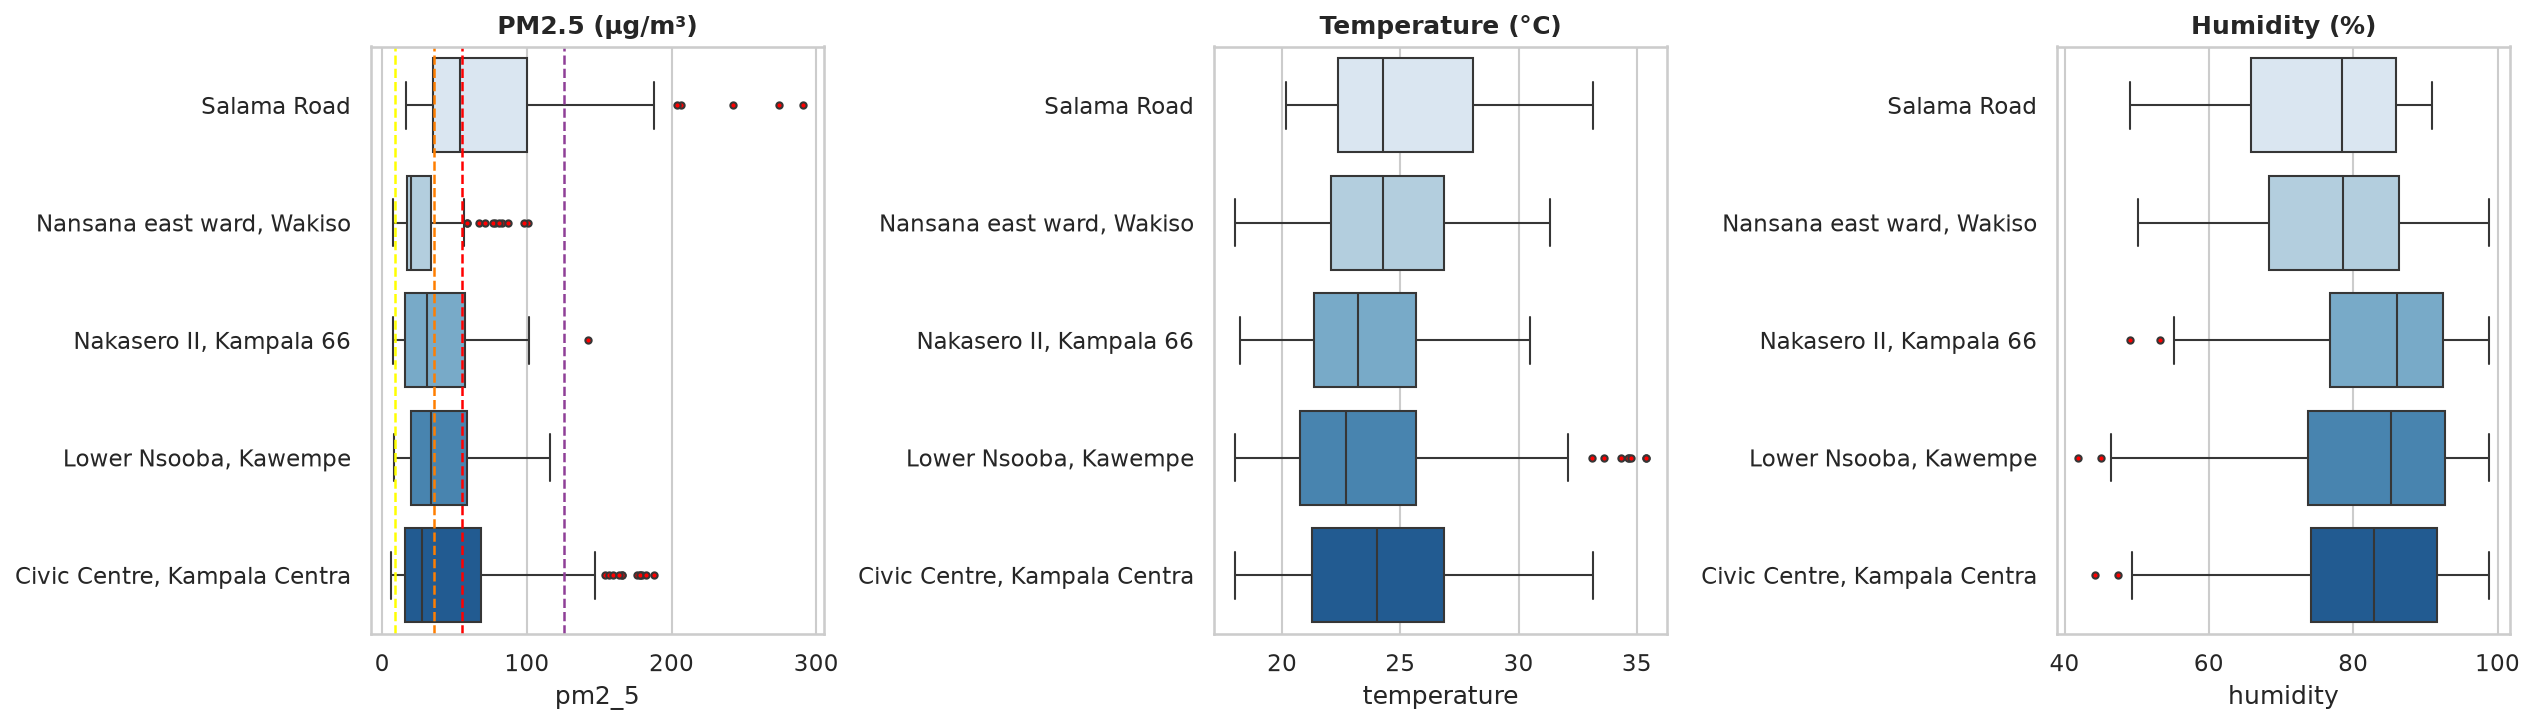
\includegraphics[width=\textwidth]{03c_boxplots.png}
\caption{Box plots per sensor; red points are 1.5$\times$IQR outliers (flagged, kept).}
\label{fig:box}
\end{figure}

\subsection{Time series with AQI bands and the diurnal cycle}
Figure~\ref{fig:ts} shows the hourly series against AQI bands for the three windows. January sits largely in the \emph{Unhealthy} and \emph{Very Unhealthy} bands, while April and June are mostly \emph{Moderate} with spikes into \emph{Unhealthy}. Every day has a morning peak (about 06:00--09:00) and an evening peak (about 19:00--23:00), with the cleanest air in the early afternoon (Figure~\ref{fig:diurnal}).

\begin{figure}[H]
\centering
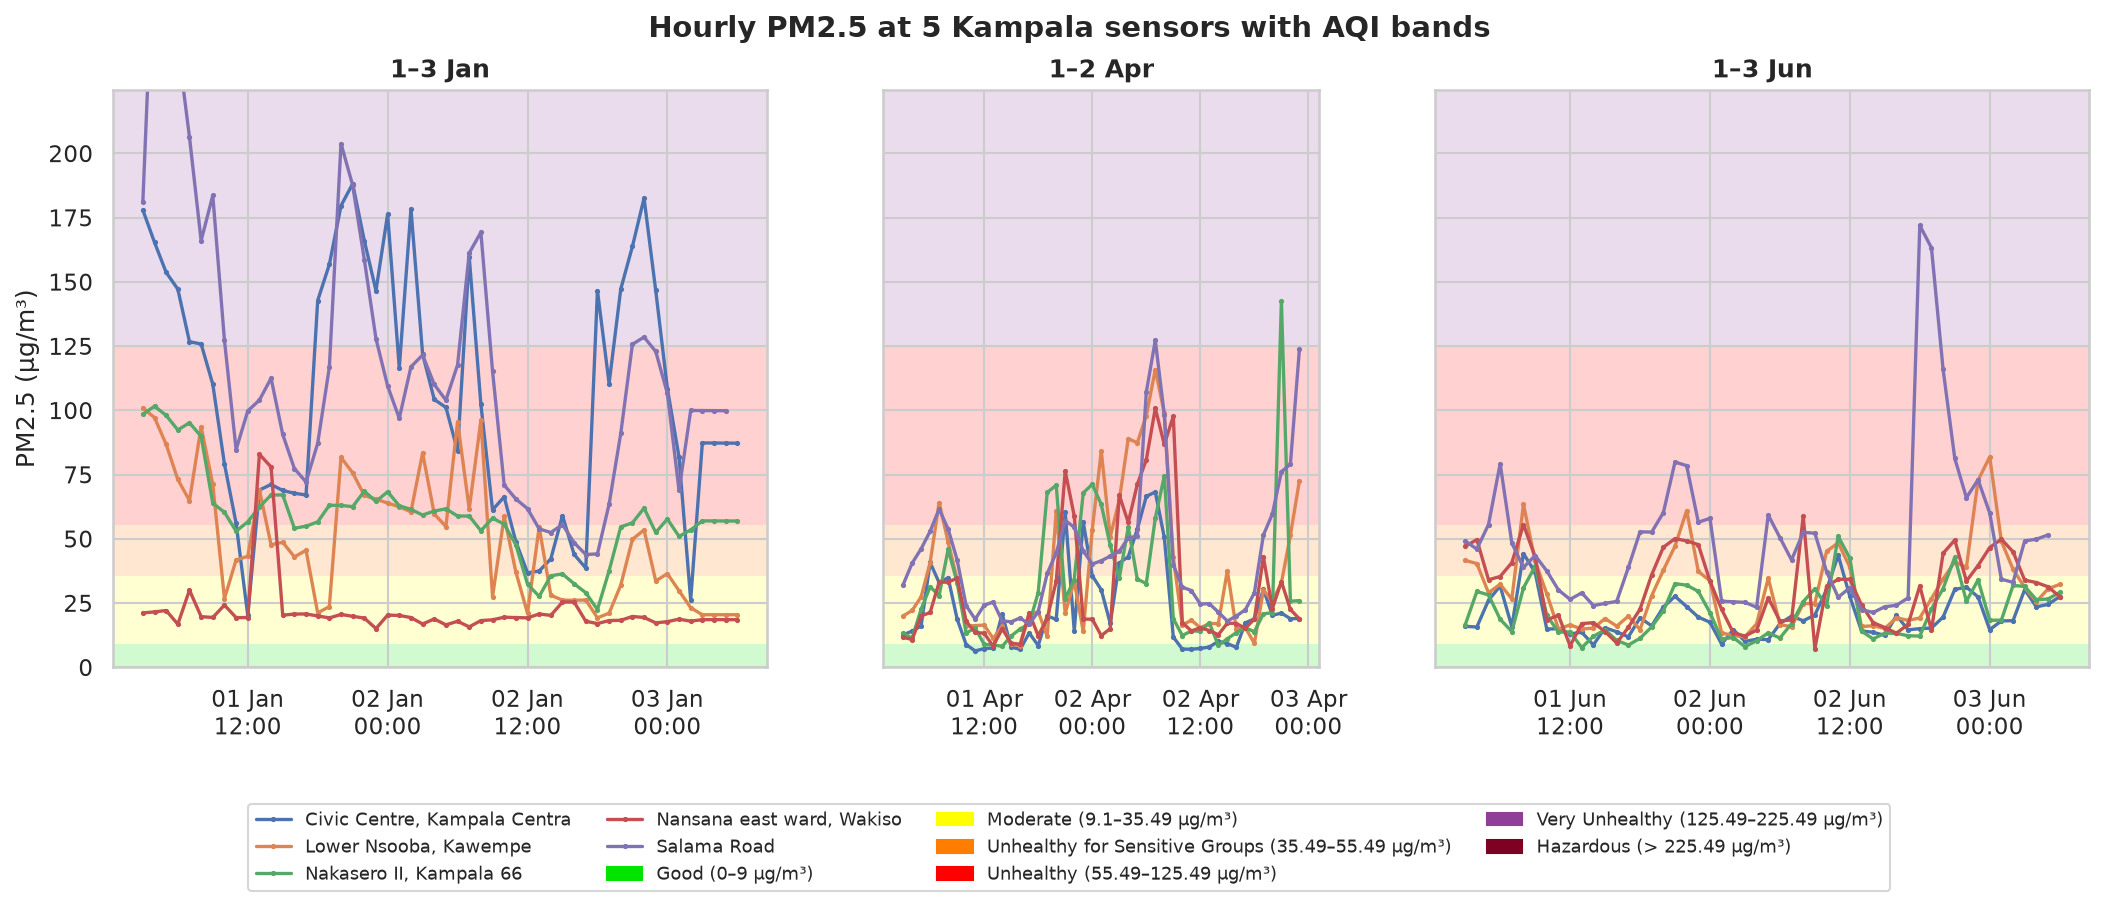
\includegraphics[width=\textwidth]{03d_timeseries_aqi.png}
\caption{Hourly PM2.5 at five Kampala sensors with AQI bands.}
\label{fig:ts}
\end{figure}

\begin{figure}[H]
\centering
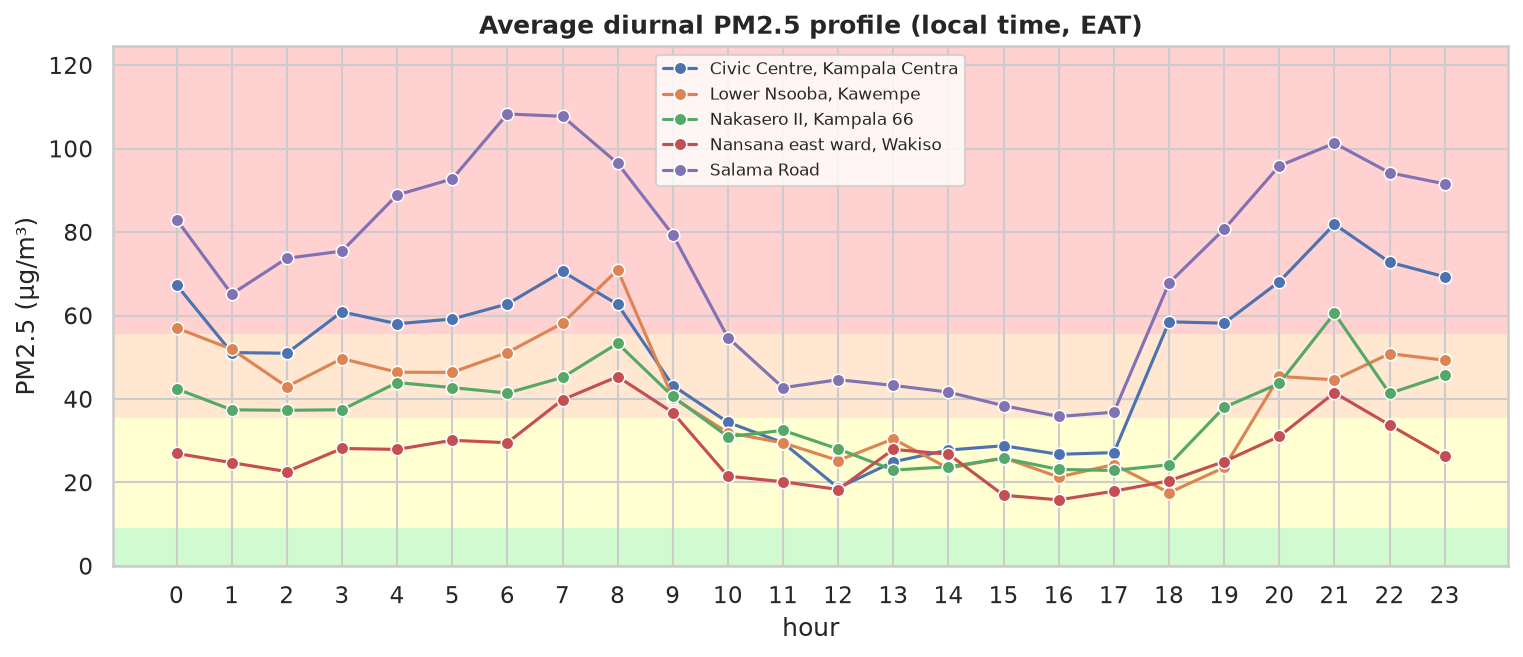
\includegraphics[width=0.85\textwidth]{03e_diurnal_profile.png}
\caption{Average diurnal PM2.5 profile (local time).}
\label{fig:diurnal}
\end{figure}

\subsection{Calendar plots}
The AQI-coloured calendar (Figure~\ref{fig:cal}) shows daily means of the unscaled, cleaned data. The full January--July calendar in the notebook is mostly grey (no data), which makes the network gaps visible at a glance; the compact version shows only the months with data. Only 0--9\% of hours are \emph{Good} at any of the five sites; about 49\% of Salama Road's hours are \emph{Unhealthy} or worse, while peri-urban Nansana is 79\% \emph{Moderate} (Figure~\ref{fig:aqishare}).

\begin{figure}[H]
\centering
\begin{subfigure}[t]{0.47\textwidth}
\centering
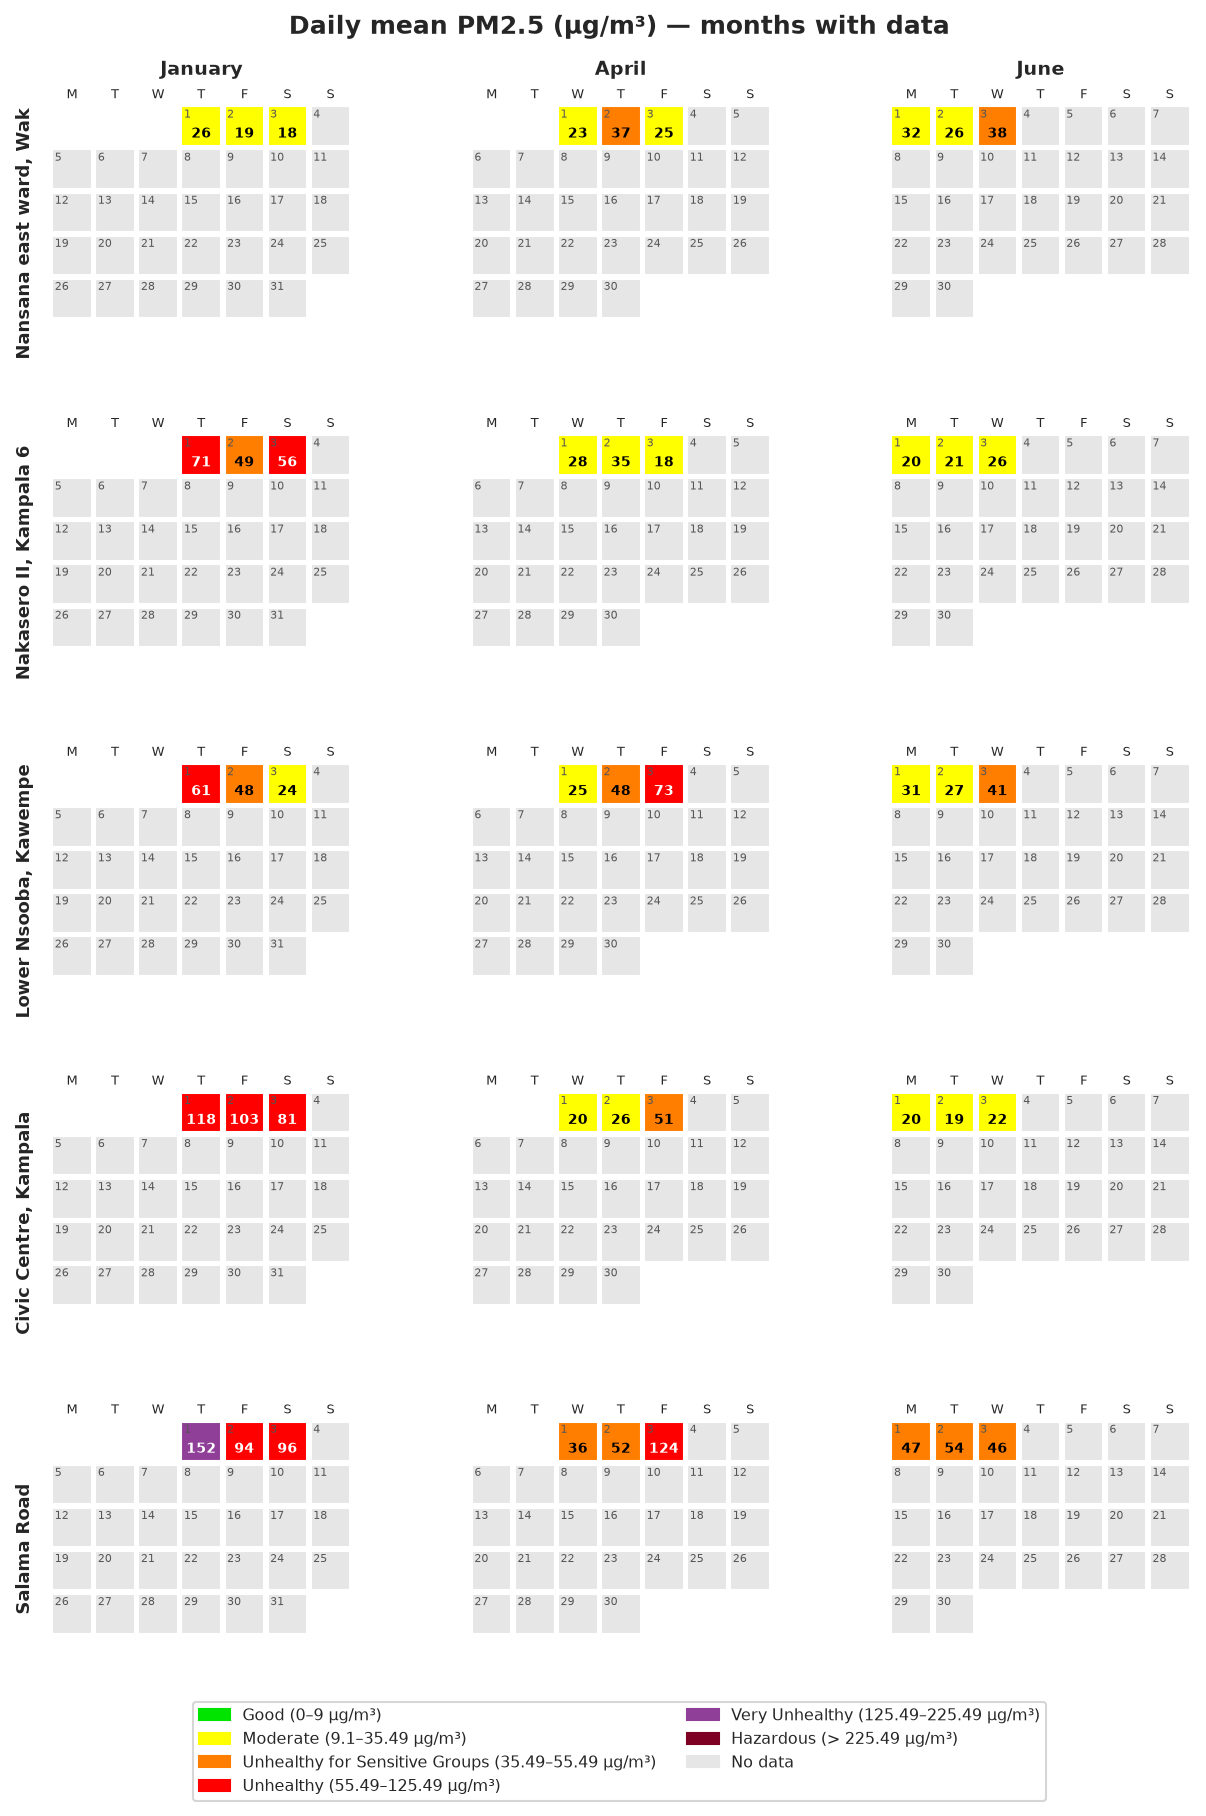
\includegraphics[width=\textwidth]{03f2_calendar_observed_months.png}
\caption{Daily mean PM2.5 (months with data).}
\label{fig:cal}
\end{subfigure}\hfill
\begin{subfigure}[t]{0.5\textwidth}
\centering
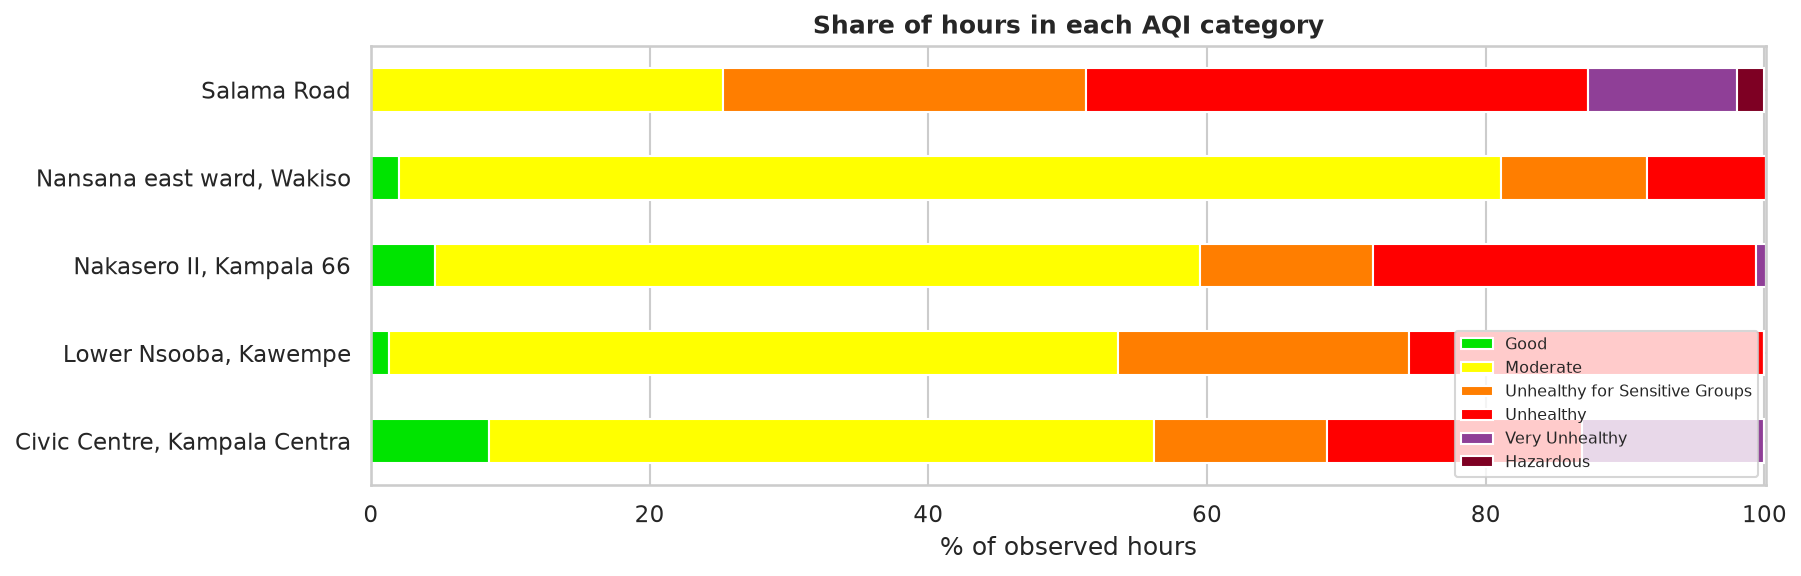
\includegraphics[width=\textwidth]{03g_aqi_share.png}
\caption{Share of observed hours per AQI category.}
\label{fig:aqishare}
\end{subfigure}
\caption{Calendar and AQI composition for the five Kampala sensors.}
\end{figure}

\subsection{Z-score transformation}
The Z-score $z = (x-\mu)/\sigma$ expresses each value as the number of standard deviations from the mean. Over all observed rows, $\mu = 32.96$\ugm{} and $\sigma = 27.73$\ugm{}. Table~\ref{tab:zthr} translates the AQI thresholds into Z units: the USG threshold lies at $z \approx 0.09$, so an above-average hour in this network is already unhealthy for sensitive groups. Z-scores range from about $-1.0$ (PM2.5 cannot be negative) to $+13.8$, so scaling re-centres and re-scales but does not remove skew; 4.7\% of hours have $|z| > 2$ and 1.5\% have $|z| > 3$, far more than a Gaussian would give. A per-sensor Z-score (each sensor's own $\mu,\sigma$) measures how unusual an hour is for that location and is useful for anomaly alerts. The model target uses the global Z-score with $\mu$ and $\sigma$ fitted on the training set only ($\mu = 34.22$, $\sigma = 28.36$\ugm), which keeps between-site differences in the target and makes the inverse transform $x = z\sigma + \mu$ straightforward.

\begin{table}[H]
\centering\small
\caption{AQI thresholds expressed as global Z-scores (EDA, all observed data).}
\label{tab:zthr}
\begin{tabular}{rlr}
\toprule
Threshold (\ugm) & Category above & Equivalent $z$ \\
\midrule
9.00 & Moderate & $-0.86$ \\
35.49 & USG & $+0.09$ \\
55.49 & Unhealthy & $+0.81$ \\
125.49 & Very Unhealthy & $+3.34$ \\
225.49 & Hazardous & $+6.94$ \\
\bottomrule
\end{tabular}
\end{table}

\begin{figure}[H]
\centering
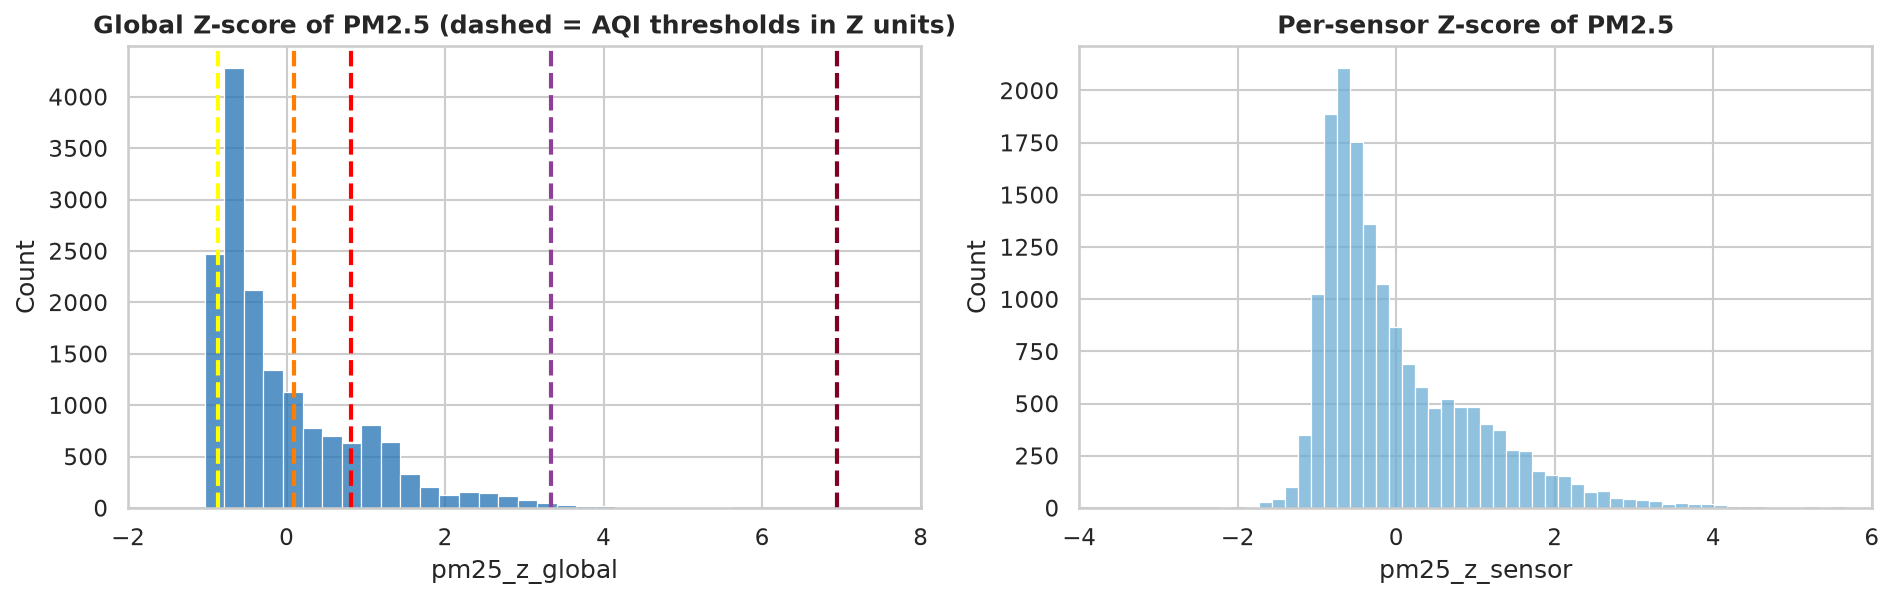
\includegraphics[width=0.95\textwidth]{03h_zscore.png}
\caption{Global (left; dashed lines are AQI thresholds in Z units) and per-sensor (right) Z-scores of PM2.5.}
\end{figure}

\subsection{Correlation with temperature and humidity}
Using only rows with measured (not imputed) weather, temperature is negatively correlated with PM2.5 and humidity positively at most sensors (Table~\ref{tab:corr}, Figure~\ref{fig:corr}). This is consistent with the physics: cool, humid nights and mornings have a shallow boundary layer that traps emissions from cooking and traffic, while the deeper afternoon boundary layer dilutes them. Correlations are weak to moderate --- close to zero at traffic-dominated Civic Centre and strongest at Salama Road --- so weather is informative but not sufficient on its own. Spearman's $\rho$ is reported alongside Pearson's $r$ because the relationship is monotonic but not linear and PM2.5 is skewed.

\begin{table}[H]
\centering\small
\caption{Correlation of temperature and humidity with PM2.5.}
\label{tab:corr}
\begin{tabular}{lrrrr}
\toprule
& \multicolumn{2}{c}{Temperature} & \multicolumn{2}{c}{Humidity} \\
\cmidrule(lr){2-3}\cmidrule(lr){4-5}
Sensor & Pearson $r$ & Spearman $\rho$ & Pearson $r$ & Spearman $\rho$ \\
\midrule
Nansana east ward & $-0.154$ & $-0.198$ & $0.238$ & $0.254$ \\
Nakasero II & $-0.141$ & $-0.144$ & $0.157$ & $0.254$ \\
Lower Nsooba & $-0.304$ & $-0.306$ & $0.334$ & $0.366$ \\
Civic Centre & $-0.082$ & $-0.096$ & $-0.014$ & $0.061$ \\
Salama Road & $-0.502$ & $-0.544$ & $0.413$ & $0.474$ \\
\midrule
All five (pooled) & $-0.187$ & $-0.197$ & $0.139$ & $0.207$ \\
\bottomrule
\end{tabular}
\end{table}

\begin{figure}[H]
\centering
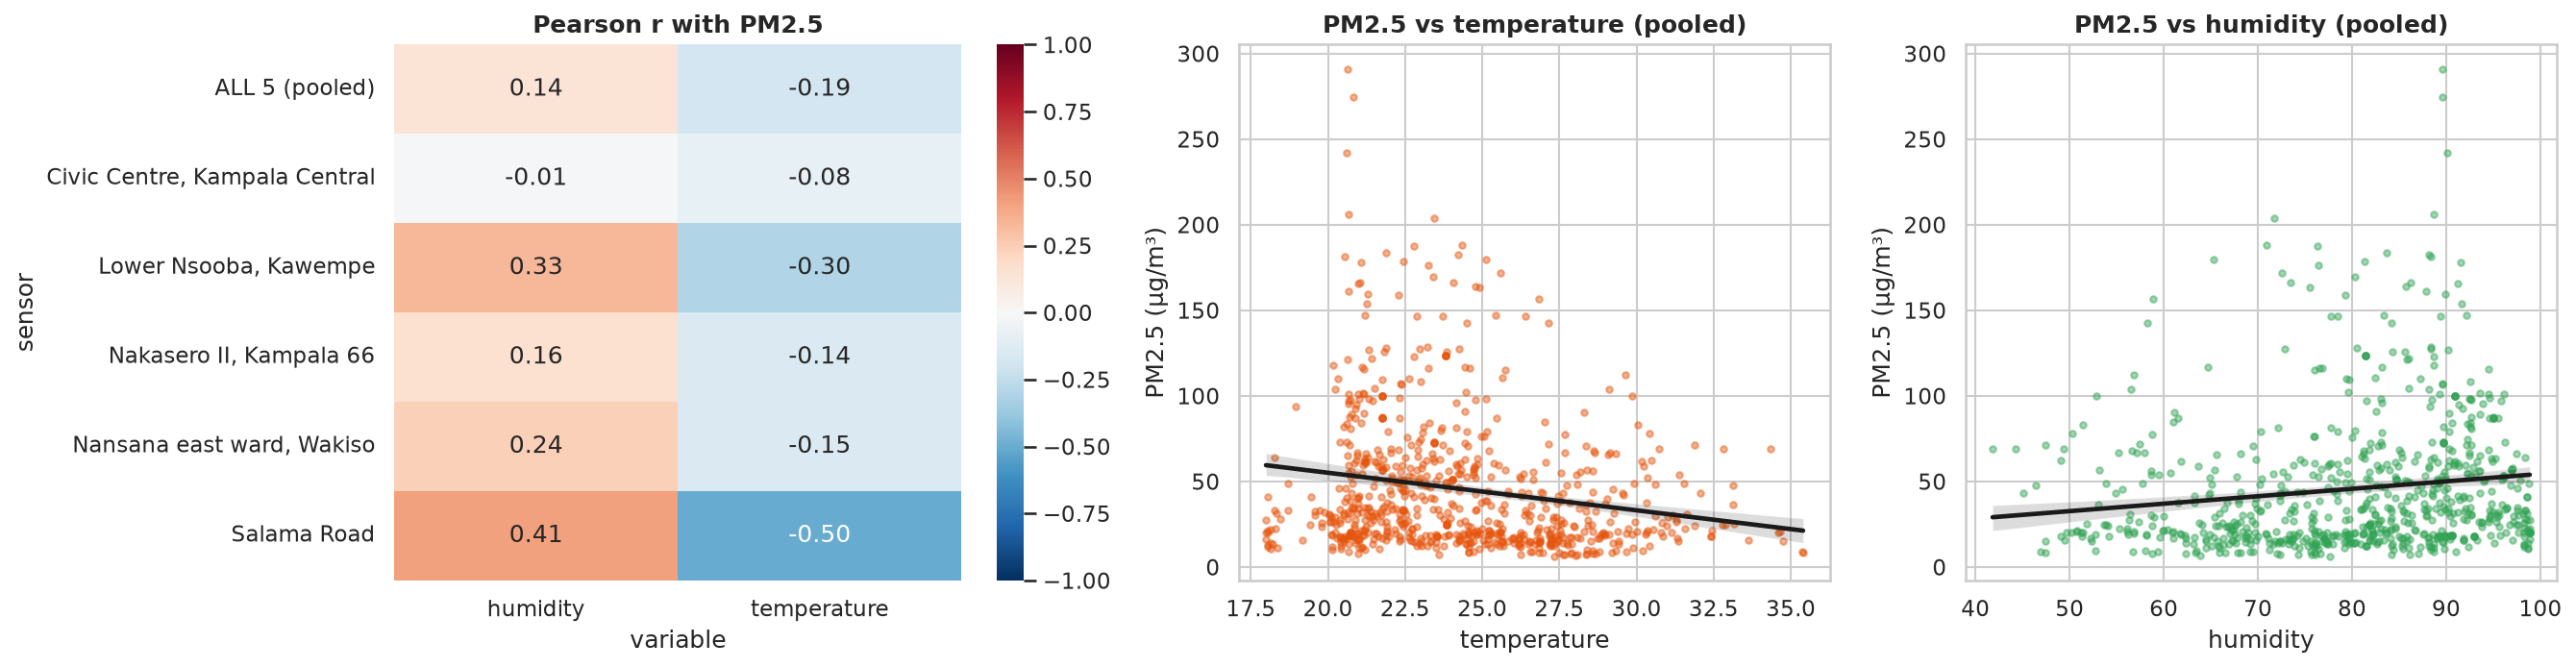
\includegraphics[width=\textwidth]{03i_correlation.png}
\caption{Pearson correlations per sensor and pooled scatter plots with linear fits.}
\label{fig:corr}
\end{figure}

% =================================================================
\section{Machine learning}
\subsection{Problem set-up}
The target is the global Z-score of hourly PM2.5. The nine features are listed in Table~\ref{tab:features}. Because PM2.5 is strongly autocorrelated, a random split would place near-identical neighbouring hours in both training and test sets and overstate performance. We therefore use a \textbf{chronological split}: the training set contains January, April and the first day of June (13{,}780 rows), and the test set is the last full 24 hours observed, 2 June 06:00 to 3 June 06:00 (2{,}468 rows). This covers a full diurnal cycle and is in the same season as the August forecast.

Hyperparameters were tuned with \texttt{RandomizedSearchCV} (15--25 candidates per model, scoring negative RMSE) using \textbf{blocked cross-validation}: \texttt{GroupKFold} with five folds and calendar days as groups \cite{roberts2017}, so whole days are held out. A plain \texttt{TimeSeriesSplit} was tried first and rejected: its early folds train only on January and validate on April, so the season flag never varies in training and tuning favours over-smoothed models. The best configuration of each model was refitted on the full training set. The test set was never used for tuning.

\subsection{Models and hyperparameters}
\begin{table}[H]
\centering\small
\caption{Models, tuned hyperparameters and selected values.}
\label{tab:models}
\begin{tabularx}{\textwidth}{L{2.4cm}L{4.5cm}L{3.5cm}Y}
\toprule
Model & Hyperparameters (search space) & Selected & Why they matter \\
\midrule
Ridge (+ polynomial) & $\alpha \in [10^{-3},10^{3}]$ (log), degree $\in\{1,2\}$ & $\alpha=98.8$, degree 2 & $\alpha$ trades variance for bias; degree 2 adds interactions such as temperature $\times$ hour \\
KNN & $k\in[3,60)$, weights, $p\in\{1,2\}$ & $k=24$, distance, $p=1$ & Small $k$ memorises noise; large $k$ over-smooths spikes; standardised features \\
SVR (RBF) & $C\in[0.1,100]$, $\gamma\in[10^{-3},1]$, $\epsilon\in[0.01,0.51]$ & $C=2.09$, $\gamma=0.031$, $\epsilon=0.071$ & $C$: penalty outside the tube; $\gamma$: kernel width; $\epsilon$: noise tolerance. Tuned on 3{,}000 rows (cost $\sim O(n^2)$) \\
Random Forest & trees 150--500, depth, min\_samples\_leaf 1--20, max\_features & 423 trees, depth none, leaf 7, features 0.4 & More trees reduce variance; depth and leaf size control overfitting; fewer features per split de-correlate trees \\
XGBoost & trees 200--900, learning rate 0.01--0.2, depth 3--8, min\_child\_weight, subsample, colsample, $\lambda$ & 204 trees, lr 0.014, depth 8, mcw 3, subsample 0.91, colsample 0.79, $\lambda=1.96$ & Learning rate $\times$ rounds sets how far boosting goes; depth and min\_child\_weight set complexity; subsampling and $\lambda$ regularise \\
Stacking ensemble & RF, XGBoost, KNN, SVR $\rightarrow$ \texttt{RidgeCV} meta-learner ($\alpha$ by internal CV) & $\alpha=31.6$; weights RF 0.36, XGB 0.53, SVR 0.22, KNN $-0.10$ & Combines models that err differently; the meta-learner learns how much to trust each \\
\bottomrule
\end{tabularx}
\end{table}

XGBoost uses CUDA automatically when a GPU is detected (e.g.\ on RunPod) and the CPU otherwise.

\subsection{Evaluation metrics}
\begin{itemize}
\item \textbf{RMSE} $=\sqrt{\tfrac{1}{n}\sum (y_i-\hat y_i)^2}$ --- the primary metric for tuning and selection. Squaring penalises large errors heavily, which suits air quality: missing a pollution spike means people are not warned. Reported in Z units and in \ugm{} (RMSE\textsubscript{\textmu g} $= \sigma\cdot$RMSE\textsubscript{z}).
\item \textbf{MAE} $=\tfrac{1}{n}\sum|y_i-\hat y_i|$ --- robust and easy to communicate. RMSE $\gg$ MAE indicates errors dominated by a few large misses.
\item \textbf{$R^2$} $=1-\sum(y_i-\hat y_i)^2/\sum(y_i-\bar y)^2$ --- share of variance explained relative to predicting the mean; negative values are worse than the mean.
\item \textbf{AQI-category accuracy} --- share of hours whose predicted AQI band matches the observed band; the metric the public experiences, but misleading under class imbalance.
\item \textbf{Not used:} MAPE is undefined or explosive on Z-scores (values cross zero) and over-penalises errors at very clean hours. For a binary health alert (e.g.\ PM2.5 $>$ 55\ugm) precision, recall and F1 would be more appropriate; if all errors mattered equally, MAE would be primary.
\end{itemize}

\subsection{Results}
Table~\ref{tab:results} and Figure~\ref{fig:compare} compare the models with two baselines: the training mean and each sensor's typical level.

\begin{table}[H]
\centering\small
\caption{Hold-out test performance (2--3 June 2026), sorted by RMSE. CV = blocked cross-validation RMSE on the training set.}
\label{tab:results}
\resizebox{\textwidth}{!}{%
\begin{tabular}{lrrrrrrrr}
\toprule
Model & RMSE$_z$ & MAE$_z$ & $R^2$ & RMSE (\ugm) & MAE (\ugm) & AQI acc.\ (\%) & CV RMSE$_z$ & Train RMSE$_z$ \\
\midrule
\textbf{XGBoost} & \textbf{0.703} & 0.432 & \textbf{0.222} & \textbf{19.95} & 12.25 & 70.9 & 0.718 & 0.517 \\
Stacking ensemble & 0.704 & 0.425 & 0.221 & 19.97 & 12.05 & 71.9 & -- & 0.582 \\
Random Forest & 0.707 & 0.424 & 0.214 & 20.05 & 12.02 & 71.3 & 0.717 & 0.501 \\
KNN & 0.732 & 0.436 & 0.157 & 20.77 & 12.38 & 69.0 & 0.746 & 0.056 \\
Ridge & 0.734 & 0.437 & 0.154 & 20.81 & 12.41 & 72.3 & 0.754 & 0.692 \\
SVR & 0.763 & 0.415 & 0.085 & 21.64 & 11.77 & 73.9 & 0.747 & 0.691 \\
\midrule
Baseline: sensor mean & 0.842 & 0.647 & $-0.114$ & 23.87 & 18.36 & 48.7 & -- & -- \\
Baseline: global mean & 0.850 & 0.664 & $-0.135$ & 24.10 & 18.84 & 72.5 & -- & -- \\
\bottomrule
\end{tabular}}
\end{table}

\begin{figure}[H]
\centering
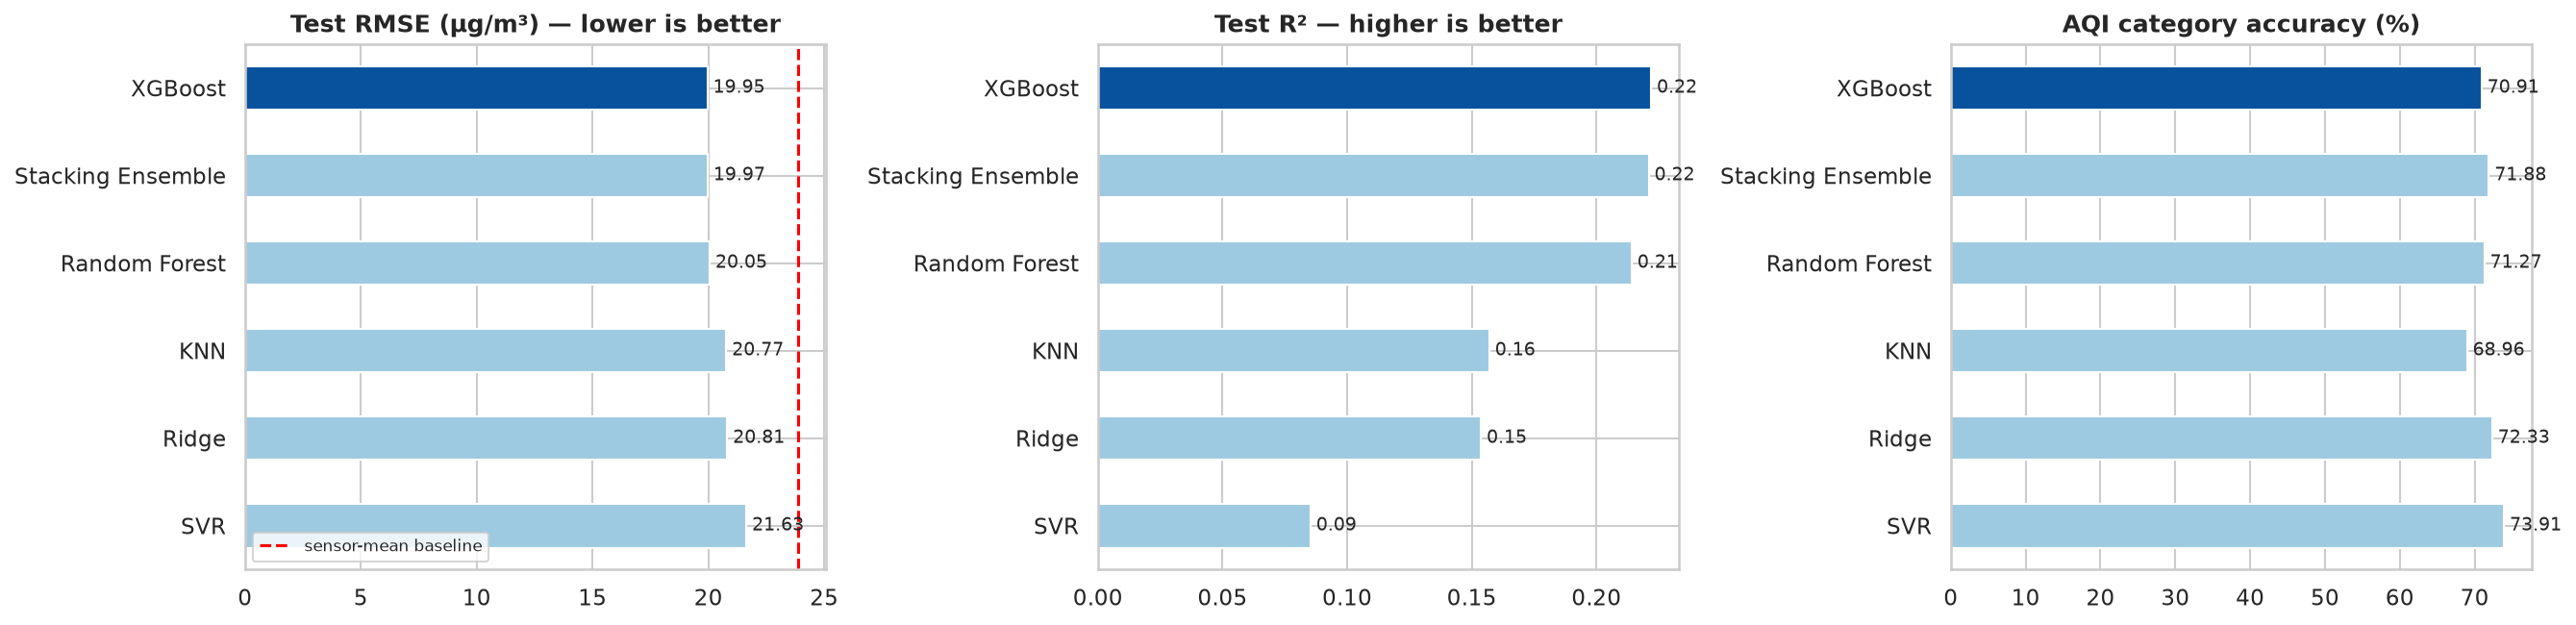
\includegraphics[width=\textwidth]{04a_model_comparison.png}
\caption{Test RMSE (dashed: sensor-mean baseline), $R^2$ and AQI accuracy.}
\label{fig:compare}
\end{figure}

\textbf{Discussion.}
\begin{itemize}
\item \textbf{XGBoost is the best model} (RMSE 19.95\ugm), with the stacking ensemble and random forest within 0.1\ugm{}. The three tree ensembles are effectively tied; XGBoost was saved because it has the lowest RMSE and is compact (1\,MB) and fast. Stacking adds little because its strongest base learners already capture the same structure.
\item \textbf{All models beat both baselines} by about 4\ugm{} of RMSE, so the features carry real information.
\item \textbf{$R^2 = 0.22$ is modest but honest.} The model has no recent observations (no lag features), only seven days of history and climatological weather at forecast time; it captures each site's typical level and the diurnal cycle, not sudden events.
\item \textbf{RMSE (20.0) $\gg$ MAE (12.3).} Errors are dominated by spikes: on test hours above 35.5\ugm{} the model under-predicts by 27.8\ugm{} on average, and on cleaner hours it over-predicts by 6.1\ugm. The model shrinks towards the middle of the distribution.
\item \textbf{Accuracy can mislead.} SVR has the highest AQI accuracy (73.9\%) but the lowest $R^2$, and the global-mean baseline reaches 72.5\% because most test hours are \emph{Moderate}.
\item \textbf{Bias--variance.} KNN overfits (train RMSE$_z$ 0.06 vs.\ test 0.73) because distance weighting reproduces training points exactly; Ridge underfits (train 0.69, test 0.73).
\end{itemize}

\subsection{Best-model diagnostics}
Figure~\ref{fig:diag} shows predicted versus observed values and residuals for XGBoost. Points flatten below the diagonal at high concentrations (largest prediction 124\ugm{} vs.\ largest observation 246\ugm), and residuals have mean $\approx 0$ but a long positive tail. The AQI confusion matrix (Figure~\ref{fig:conf}) shows that 1{,}676 of 1{,}790 \emph{Moderate} hours are classified correctly, but of the 456 hours that were USG or worse, only 32\% are predicted as USG or worse (recall), with 55\% precision. For an early-warning service, a lower alert threshold would raise recall at the cost of more false alarms.

\begin{figure}[H]
\centering
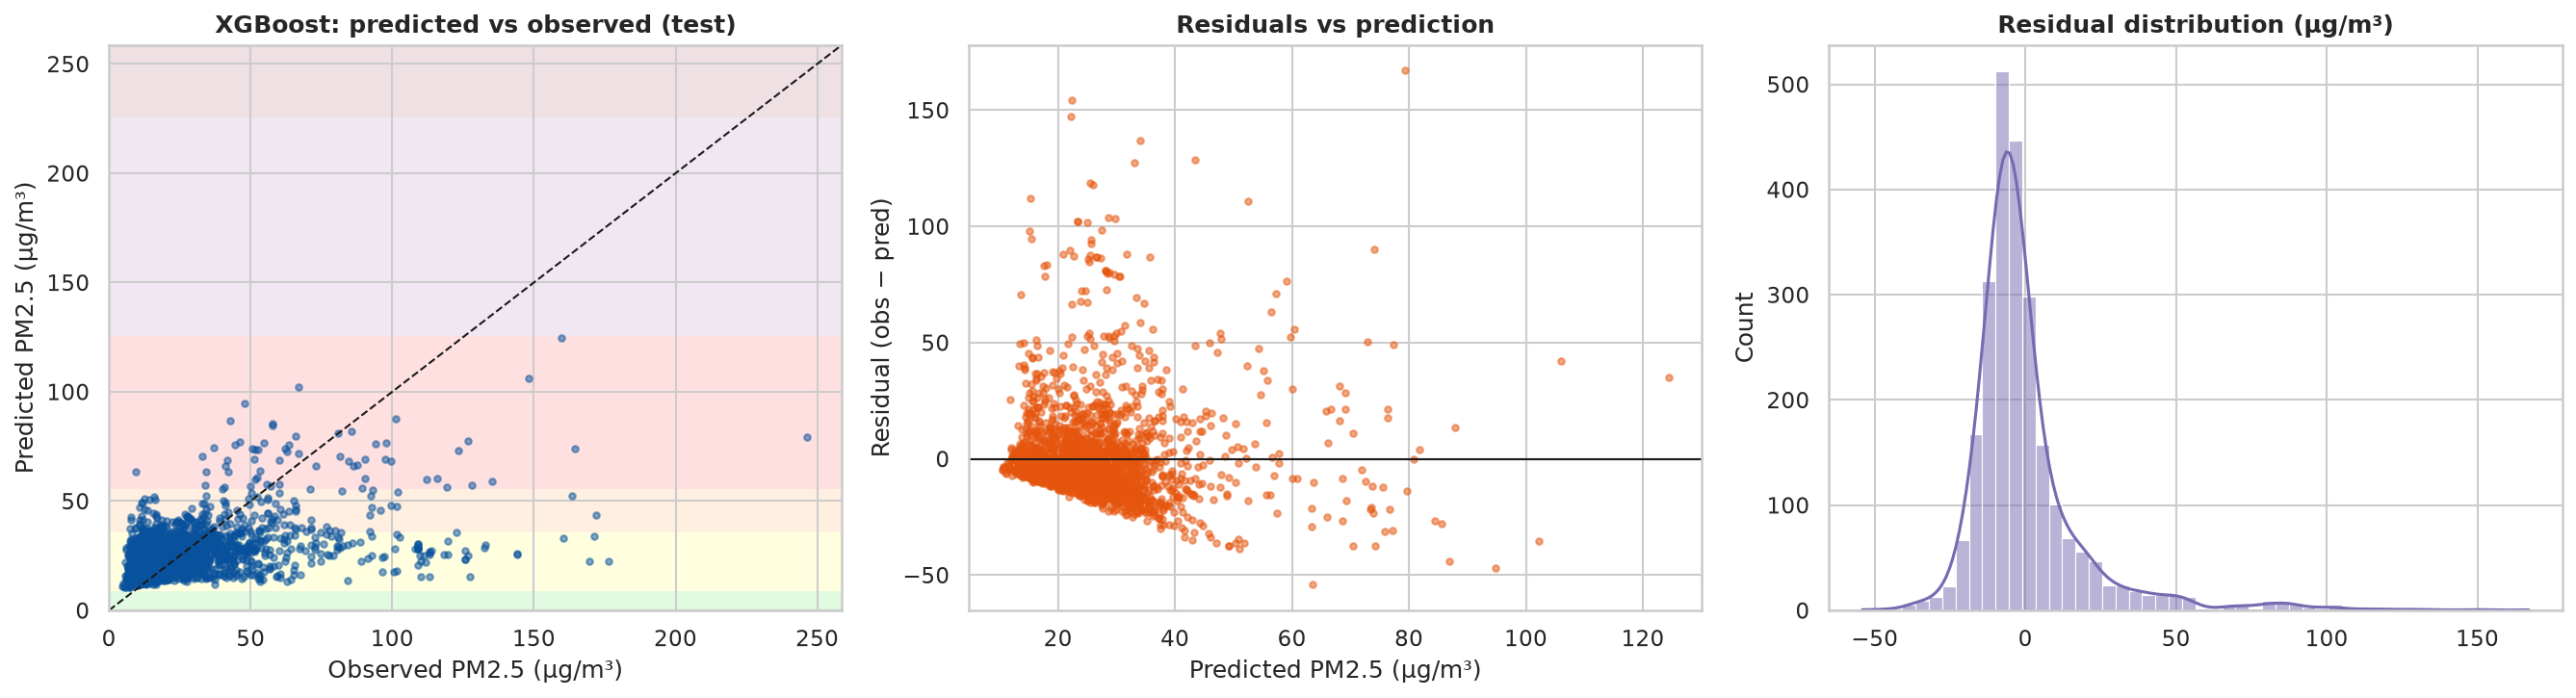
\includegraphics[width=\textwidth]{04b_best_model_diagnostics.png}
\caption{XGBoost on the test set: predicted vs.\ observed (AQI-shaded), residuals vs.\ prediction, and residual distribution.}
\label{fig:diag}
\end{figure}

\begin{figure}[H]
\centering
\begin{subfigure}[t]{0.42\textwidth}
\centering
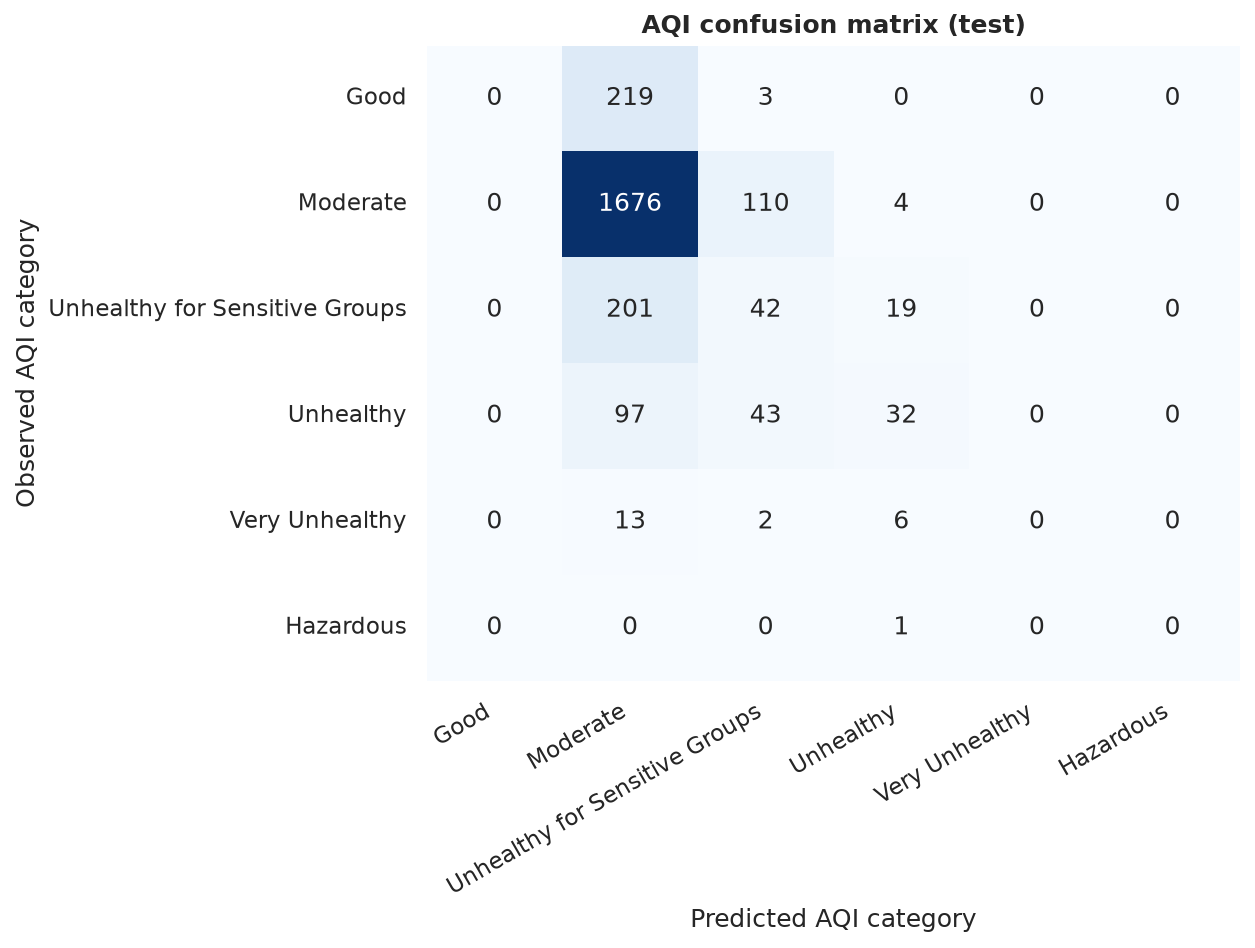
\includegraphics[width=\textwidth]{04c_aqi_confusion.png}
\caption{AQI confusion matrix (test).}
\label{fig:conf}
\end{subfigure}\hfill
\begin{subfigure}[t]{0.55\textwidth}
\centering
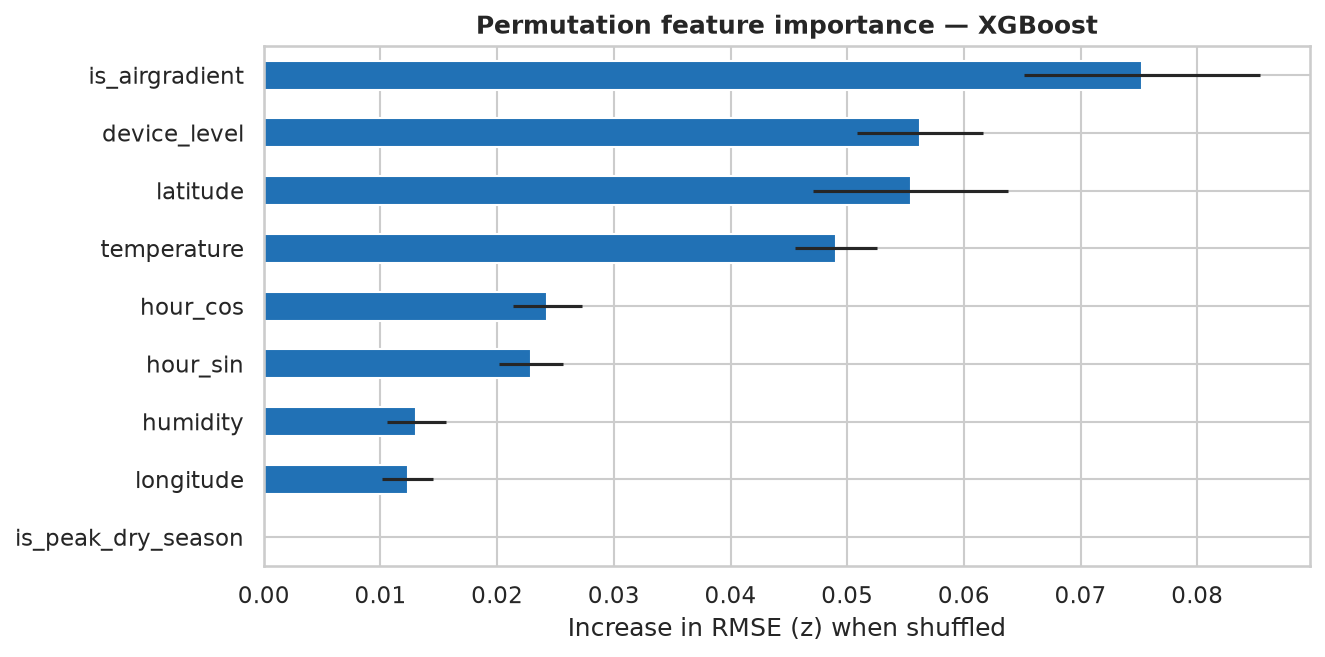
\includegraphics[width=\textwidth]{04d_feature_importance.png}
\caption{Permutation importance (increase in test RMSE$_z$).}
\label{fig:fi}
\end{subfigure}
\caption{Classification view and feature importance of the best model.}
\end{figure}

Permutation importance (Figure~\ref{fig:fi}) ranks \texttt{is\_airgradient} first: the AirGradient sensors in the test day are much more polluted (mean 57.8 vs.\ 24.4\ugm{} for AirQo devices), so the flag acts as a marker for a group of very polluted sites. Device level and latitude (where) follow, then temperature and hour of day (when, and under what weather). The season flag scores zero only because it is constant in the June test day; shuffling a constant changes nothing.

\subsection{Saved model}
The best model is serialised with \texttt{joblib} as \texttt{models/best\_pm25\_model.joblib}. The artifact bundles the fitted model, the feature list, the target scaler ($\mu$, $\sigma$) for the inverse transform, the device encodings, the weather climatology used for forecasting, sensor metadata, AQI definitions, hyperparameters and test metrics. A human-readable model card is saved as \texttt{models/best\_model\_card.json}; the stacking ensemble is also saved.

% =================================================================
\section{Forecasting August 2026}
\subsection{Procedure}
The saved artifact is re-loaded from disk to show that it works on its own. Future rows are built for every sensor: hourly from 1 to 16 August 2026 for the daily forecast (covering both ``1--14 August'' and the full calendar weeks Monday 3 to Sunday 16 August) and the 24 hours of Saturday 1 August for the hourly forecast. Hour, coordinates, device level, network and the season flag (August $=$ non-peak) are known in advance. Temperature and humidity are not, so each sensor's June hour-of-day mean is used --- June is the closest observed month to August --- with April values and then the network hour mean as fall-backs. Predictions are inverse-transformed,
\begin{equation}
\widehat{\text{PM2.5}} = \max\!\left(0,\; \hat z\,\sigma + \mu\right), \qquad \sigma = 28.36,\; \mu = 34.22\ \text{\ugm},
\end{equation}
and daily values are the mean of the 24 hourly predictions. Each prediction is reported with a $\pm1$ test-RMSE band ($\approx\pm20$\ugm). All forecasts are saved under \texttt{outputs/forecasts/}.

\subsection{Results}
Across all 149 sensors and 16 days, 92.6\% of sensor-days are forecast \emph{Moderate}, 6.0\% \emph{USG} and 1.3\% \emph{Unhealthy}. Figures~\ref{fig:fccal}--\ref{fig:fchour} show five sensors chosen to balance zones: Kampala Central (Civic Centre), Kampala Metro (Nansana), Jinja (Main Street), Mbarara (University) and Gulu (Layibi). Central Kampala is highest (29\ugm{} daily mean) and Gulu lowest (16\ugm).

Because none of the inputs change from one August day to the next, each sensor's daily forecast is almost constant: the model produces a \emph{climatological} forecast --- the expected level for that site, hour and season. Day-to-day variation would come from feeding real weather forecasts into the same model. The hourly forecast for 1 August shows the morning peak (06:00--08:00) and the evening rise (around 21:00); Civic Centre reaches about 45\ugm{} (USG) at 06:00, and air is cleanest at midday.

\begin{figure}[H]
\centering
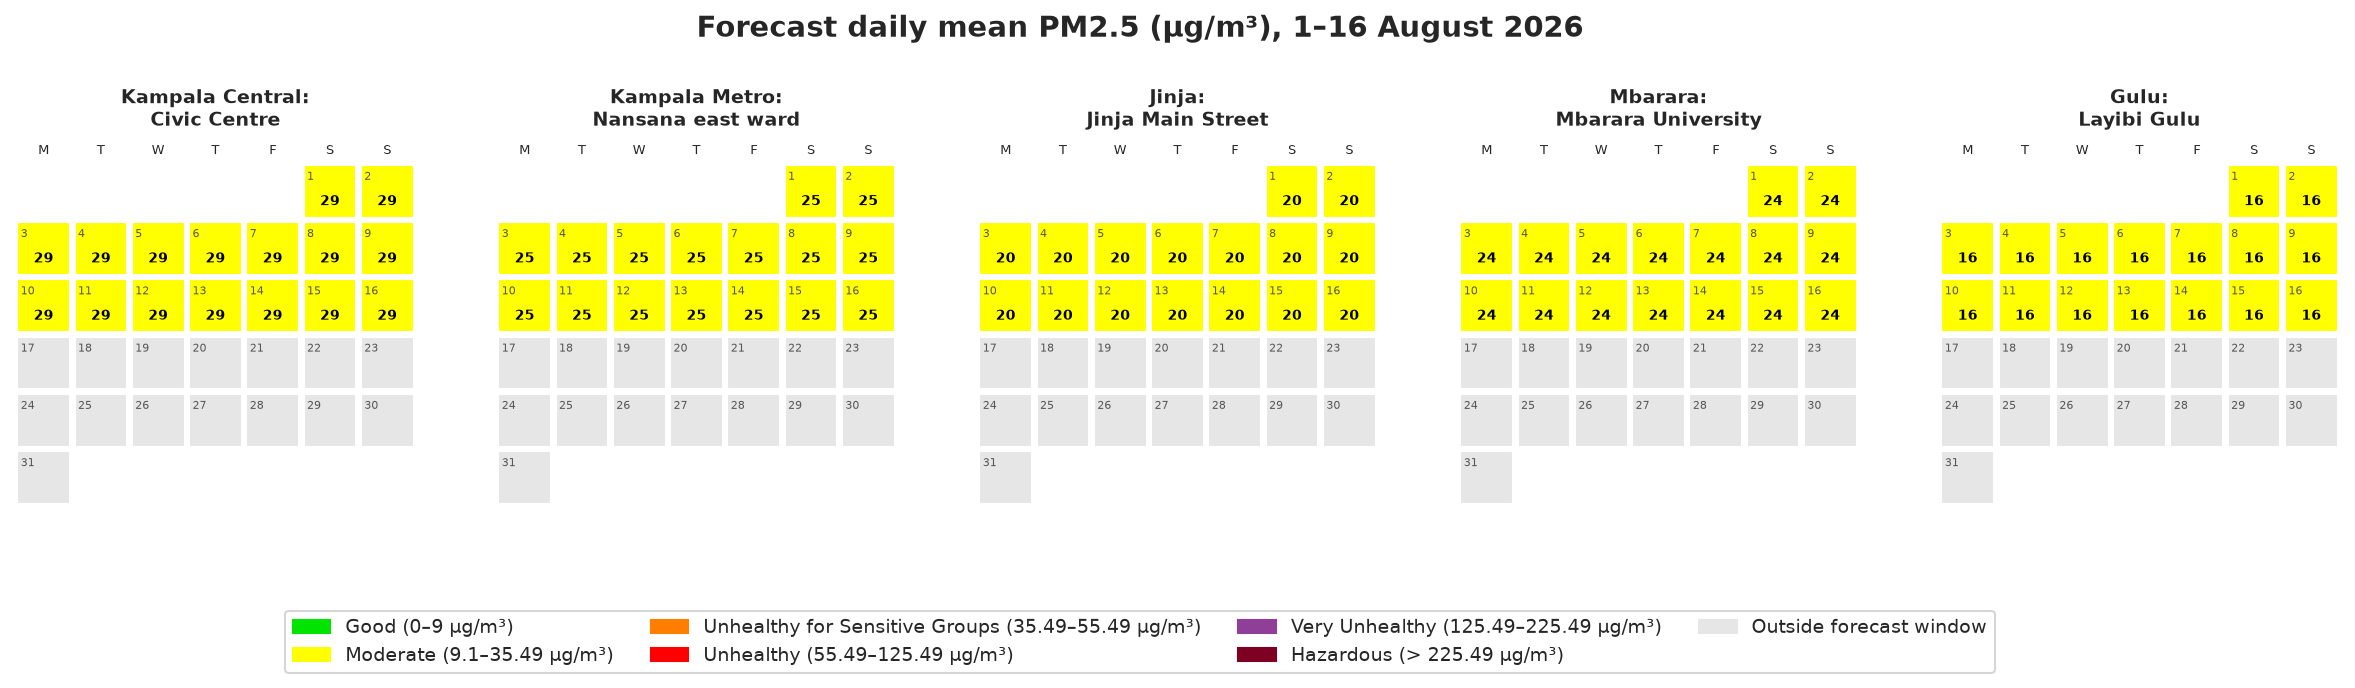
\includegraphics[width=\textwidth]{05a_forecast_calendar.png}
\caption{Calendar of forecast daily mean PM2.5, 1--16 August 2026, with the AQI legend.}
\label{fig:fccal}
\end{figure}

\begin{figure}[H]
\centering
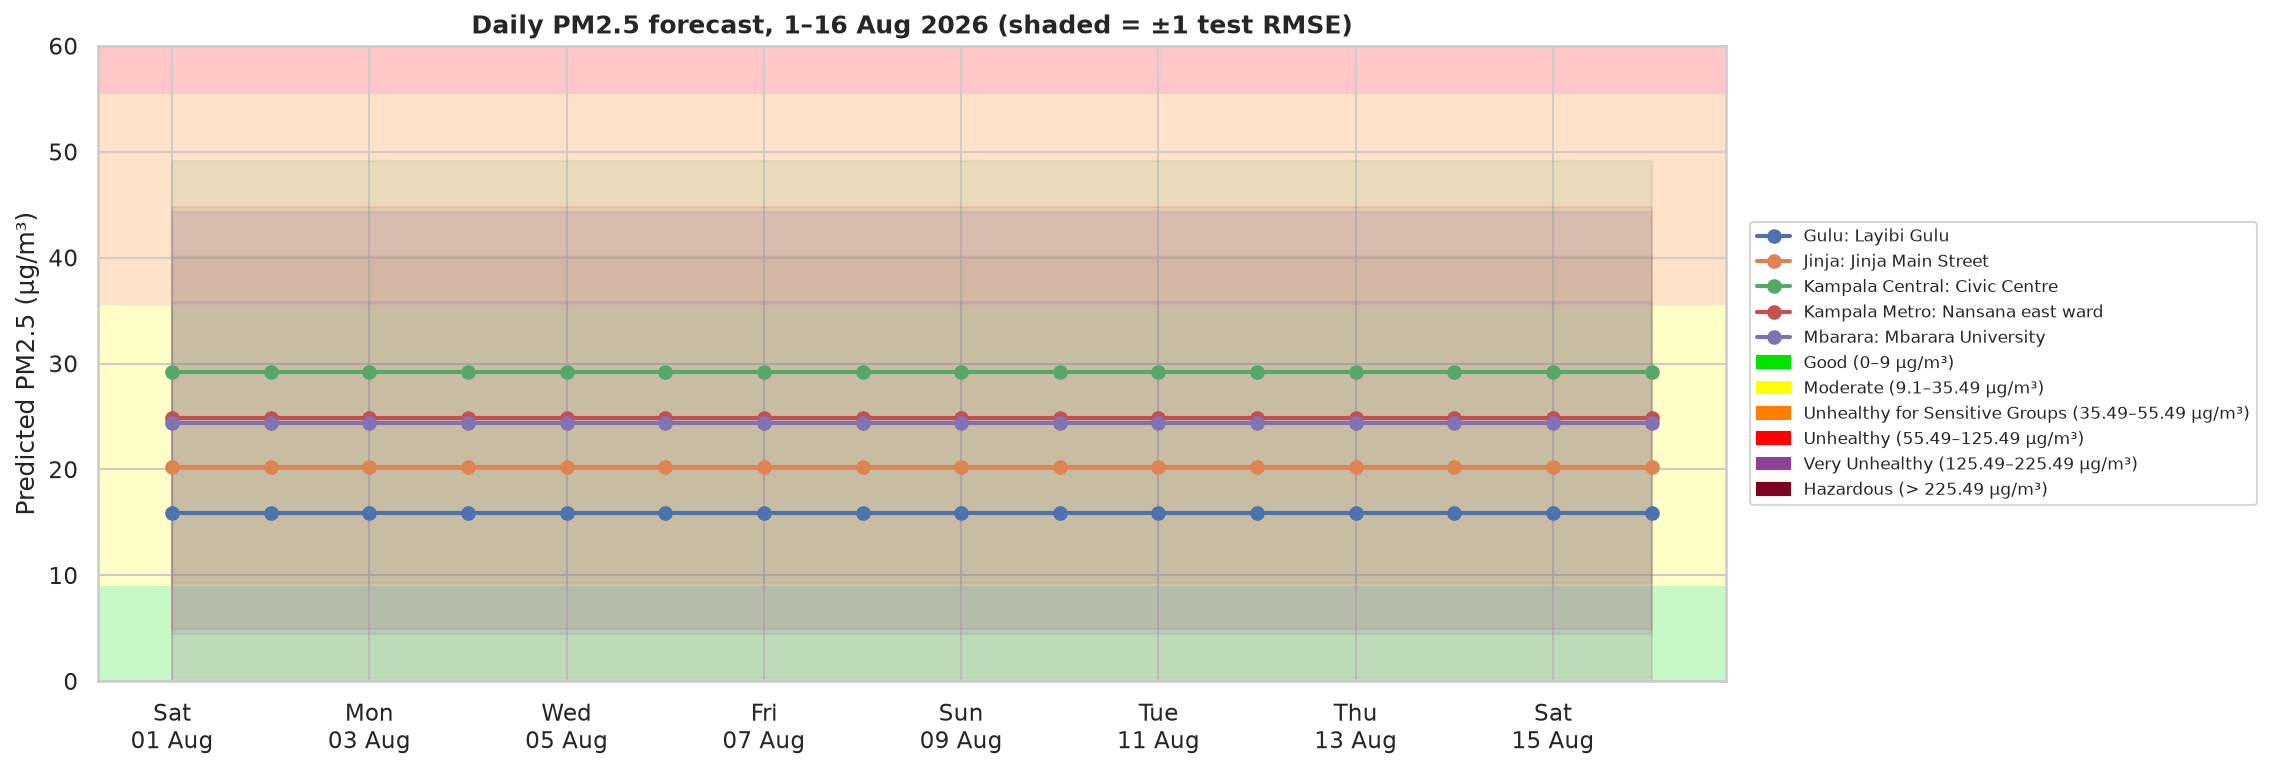
\includegraphics[width=\textwidth]{05b_forecast_daily_timeseries.png}
\caption{Daily forecast time series with AQI bands; shading is $\pm1$ test RMSE.}
\label{fig:fcdaily}
\end{figure}

\begin{figure}[H]
\centering
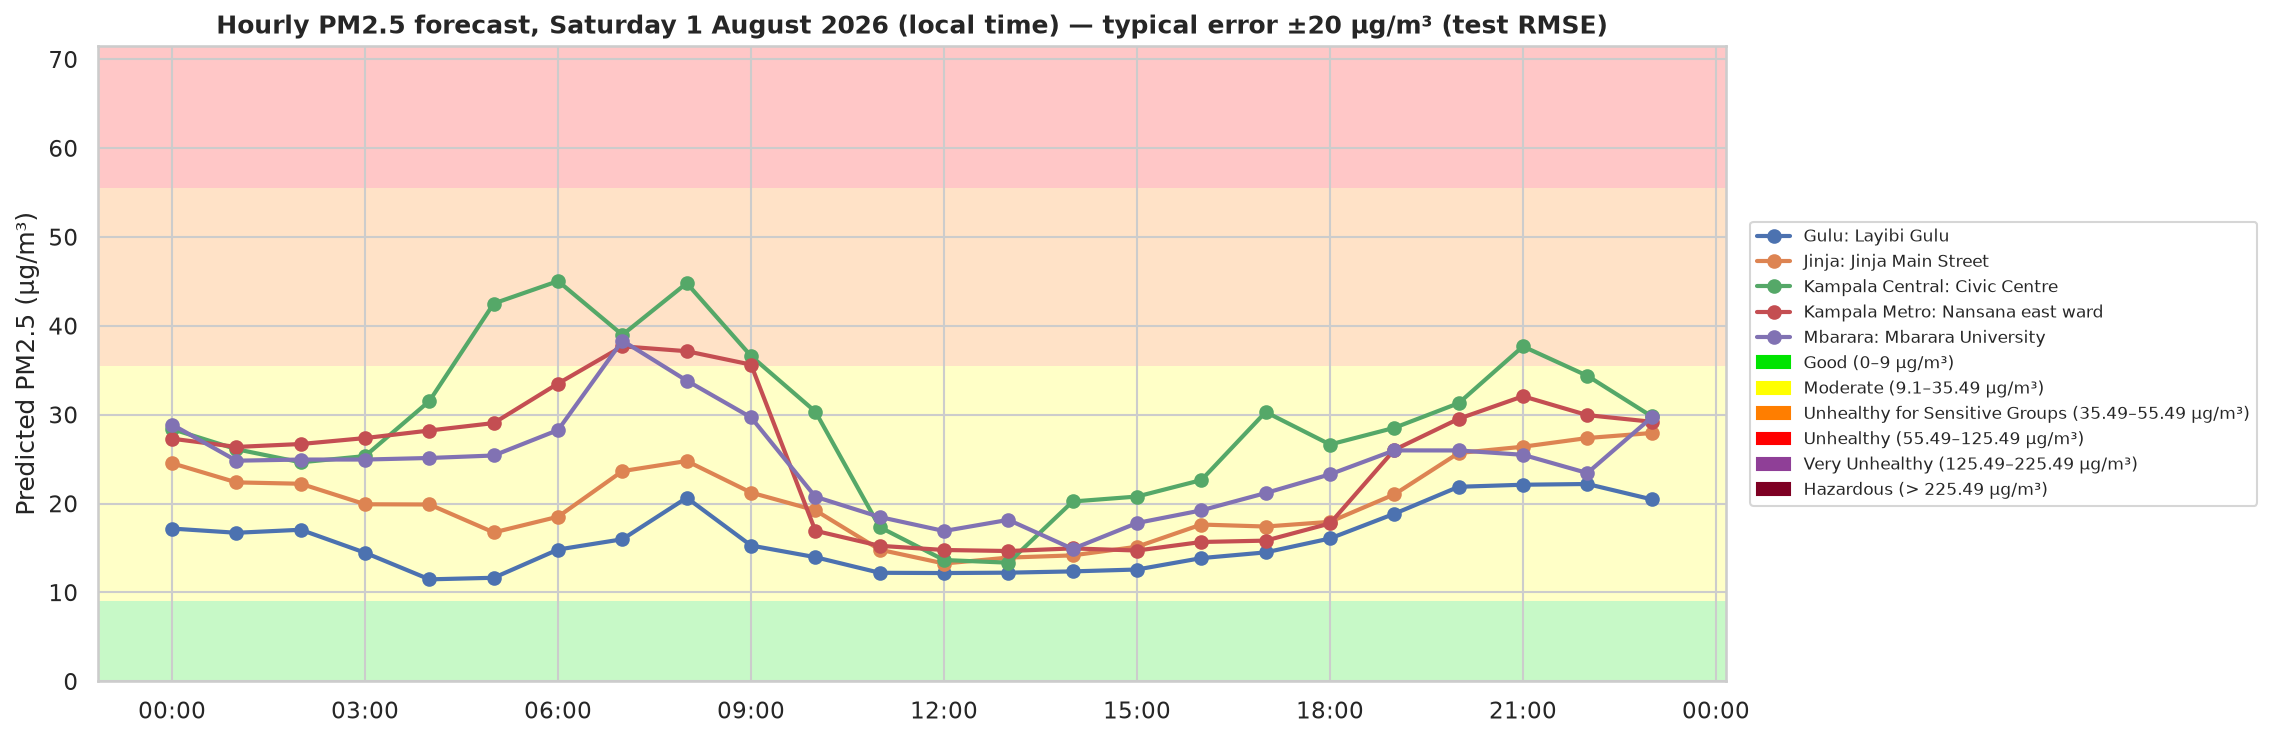
\includegraphics[width=\textwidth]{05c_forecast_hourly_aug01.png}
\caption{Hourly forecast for 1 August 2026 (local time) with AQI bands.}
\label{fig:fchour}
\end{figure}

\subsection{Bonus: map of at-risk sensors at 13:00 on 1 August}
Using Natural Earth shapefiles of Uganda's boundary, districts and lakes (stored in \texttt{data/shapefiles/}), Figure~\ref{fig:map} maps the sensors forecast in the USG to Very Unhealthy range (35.5--225.5\ugm) at 13:00 on 1 August. Only 2 of 149 sensors qualify --- Sir Apollo Kagwa Road (50\ugm) and Kamwokya Primary School (37\ugm), both in central Kampala --- because 13:00 is near the daily minimum, when the boundary layer is deepest. The same map at 07:00 or 21:00 would show many more sites at risk.

\begin{figure}[H]
\centering
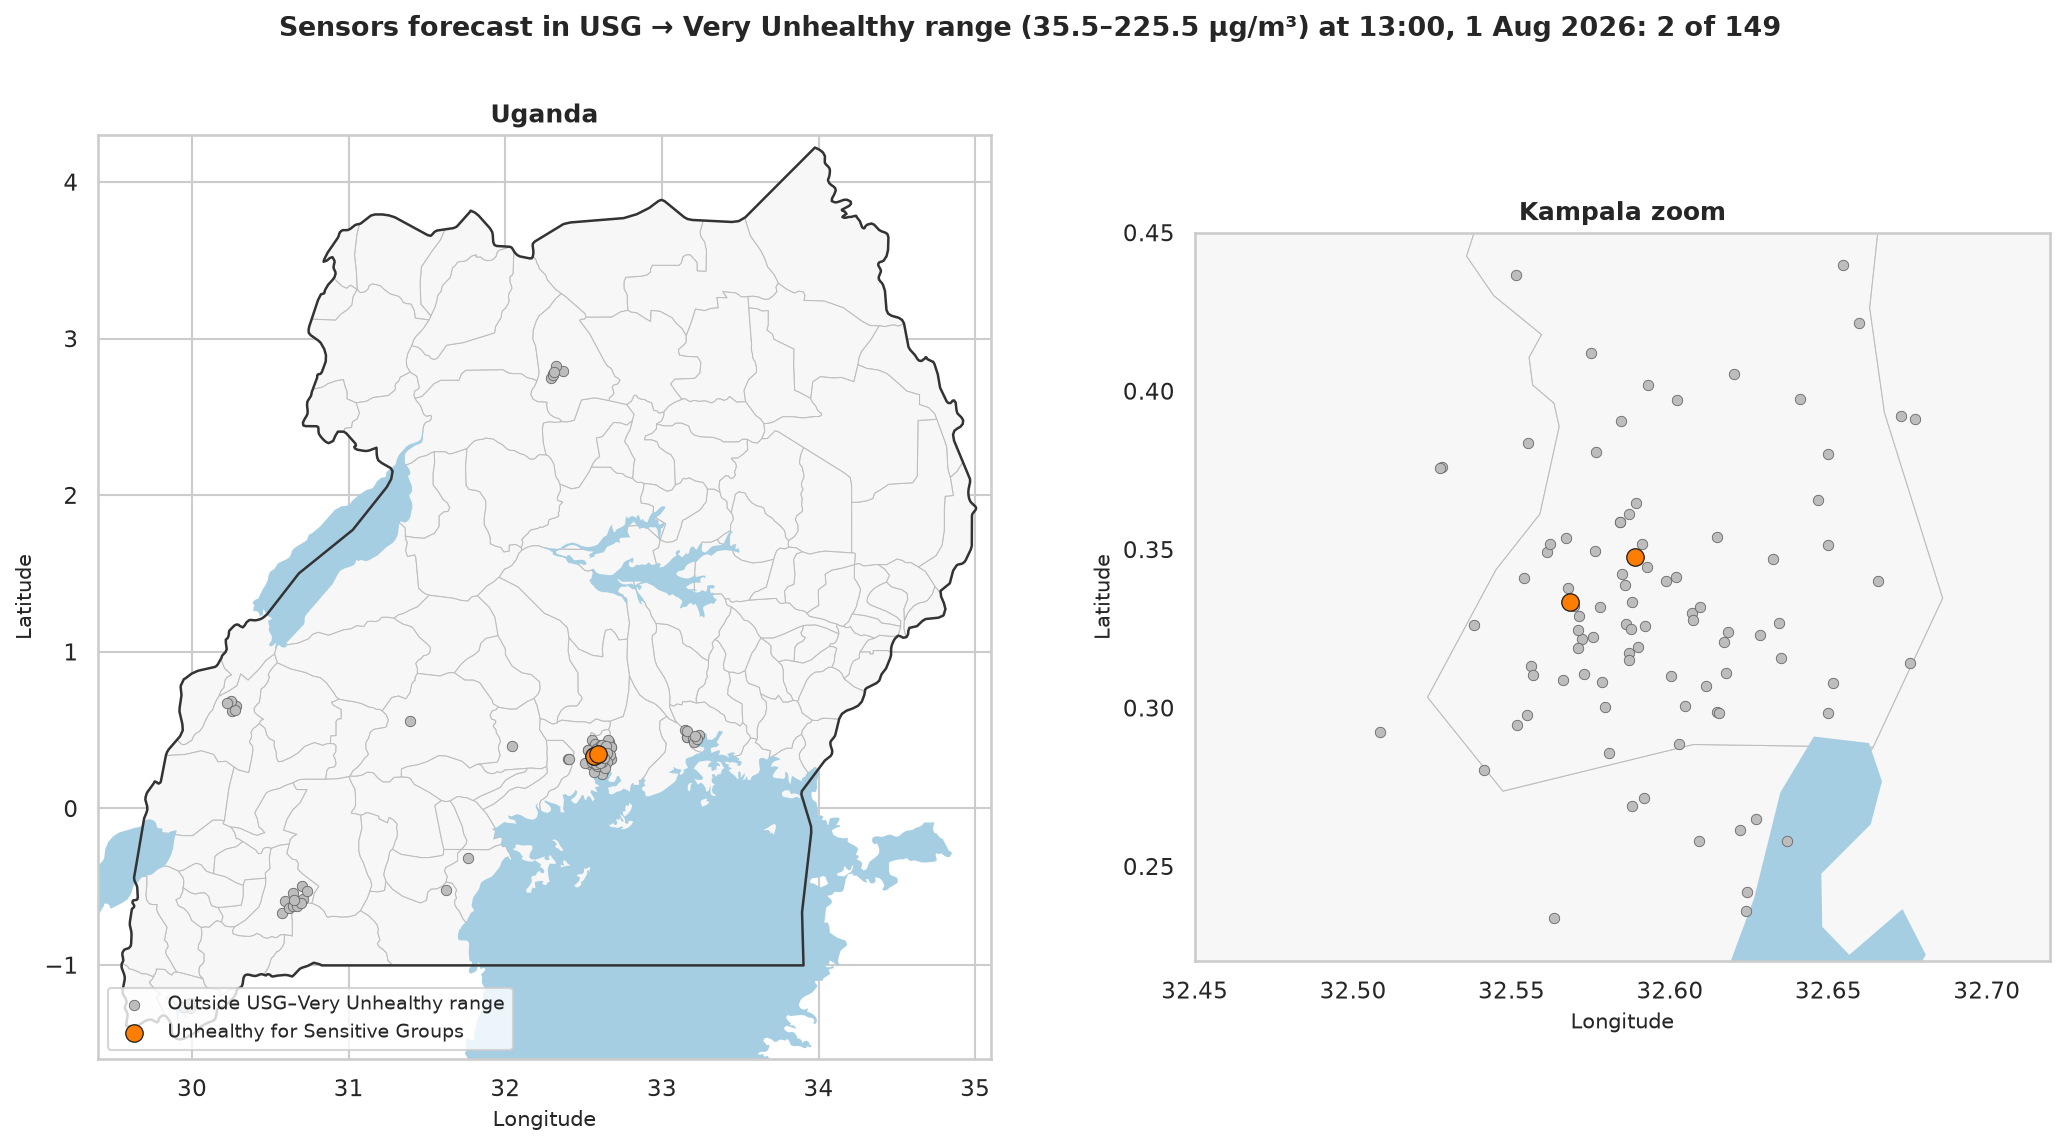
\includegraphics[width=0.95\textwidth]{05e_bonus_map_13h.png}
\caption{Sensors forecast in the USG--Very Unhealthy range at 13:00, 1 August 2026.}
\label{fig:map}
\end{figure}

% =================================================================
\section{Model monitoring with Evidently AI}
\subsection{What Evidently measures}
Evidently (v0.7) compares a \emph{reference} dataset with a \emph{current} one. We used the training period as reference and the test day as current, plus a seasonal comparison of January (dry) against April (wet).
\begin{itemize}
\item \textbf{Data drift} --- whether the distribution of each input feature has changed. For numeric columns with more than 1{,}000 rows Evidently uses the \emph{normalised Wasserstein distance} (drift if $>0.1$, i.e.\ the distribution has moved by more than 0.1 standard deviations); for smaller samples the Kolmogorov--Smirnov test (drift if $p<0.05$); for categorical or binary columns the Jensen--Shannon distance (drift if $>0.1$). The dataset is flagged as drifted when at least 50\% of columns drift.
\item \textbf{Target drift} --- the same tests on the true PM2.5 Z-score: the pollution regime itself has changed (concept-drift risk).
\item \textbf{Prediction drift} --- the same tests on the model's outputs.
\item \textbf{Model drift (performance)} --- \texttt{RegressionPreset} reports RMSE, MAE, mean error (bias), MAPE, $R^2$ and maximum absolute error for each dataset; deterioration on current data is model drift.
\end{itemize}

\subsection{Results}
\begin{table}[H]
\centering\small
\caption{Evidently drift scores (Wasserstein distance, normalised, except JS = Jensen--Shannon). Bold = drift detected.}
\label{tab:drift}
\begin{tabular}{lrrL{6.3cm}}
\toprule
Column & Train $\rightarrow$ test & Jan $\rightarrow$ Apr & Interpretation \\
\midrule
hour\_sin / hour\_cos & 0.044 / 0.074 & 0.046 / 0.027 & All hours covered: monitoring window complete \\
latitude / longitude & 0.036 / 0.050 & 0.040 / 0.069 & Stable spatial coverage \\
device\_level & 0.076 & 0.097 & Stable mix of online sensors \\
is\_airgradient (JS) & 0.024 & 0.089 & Stable hardware mix \\
temperature & \textbf{0.268} & \textbf{0.119} & Seasonal weather shift: model extrapolating \\
humidity & \textbf{0.314} & \textbf{0.355} & Wet season much more humid \\
is\_peak\_dry\_season (JS) & \textbf{0.413} & \textbf{0.833} & By construction (season flag) \\
target & \textbf{0.294} & \textbf{0.784} & Pollution regime changed (January far dirtier) \\
prediction & \textbf{0.416} & \textbf{1.012} & Outputs follow the inputs \\
\bottomrule
\end{tabular}
\end{table}

\begin{figure}[H]
\centering
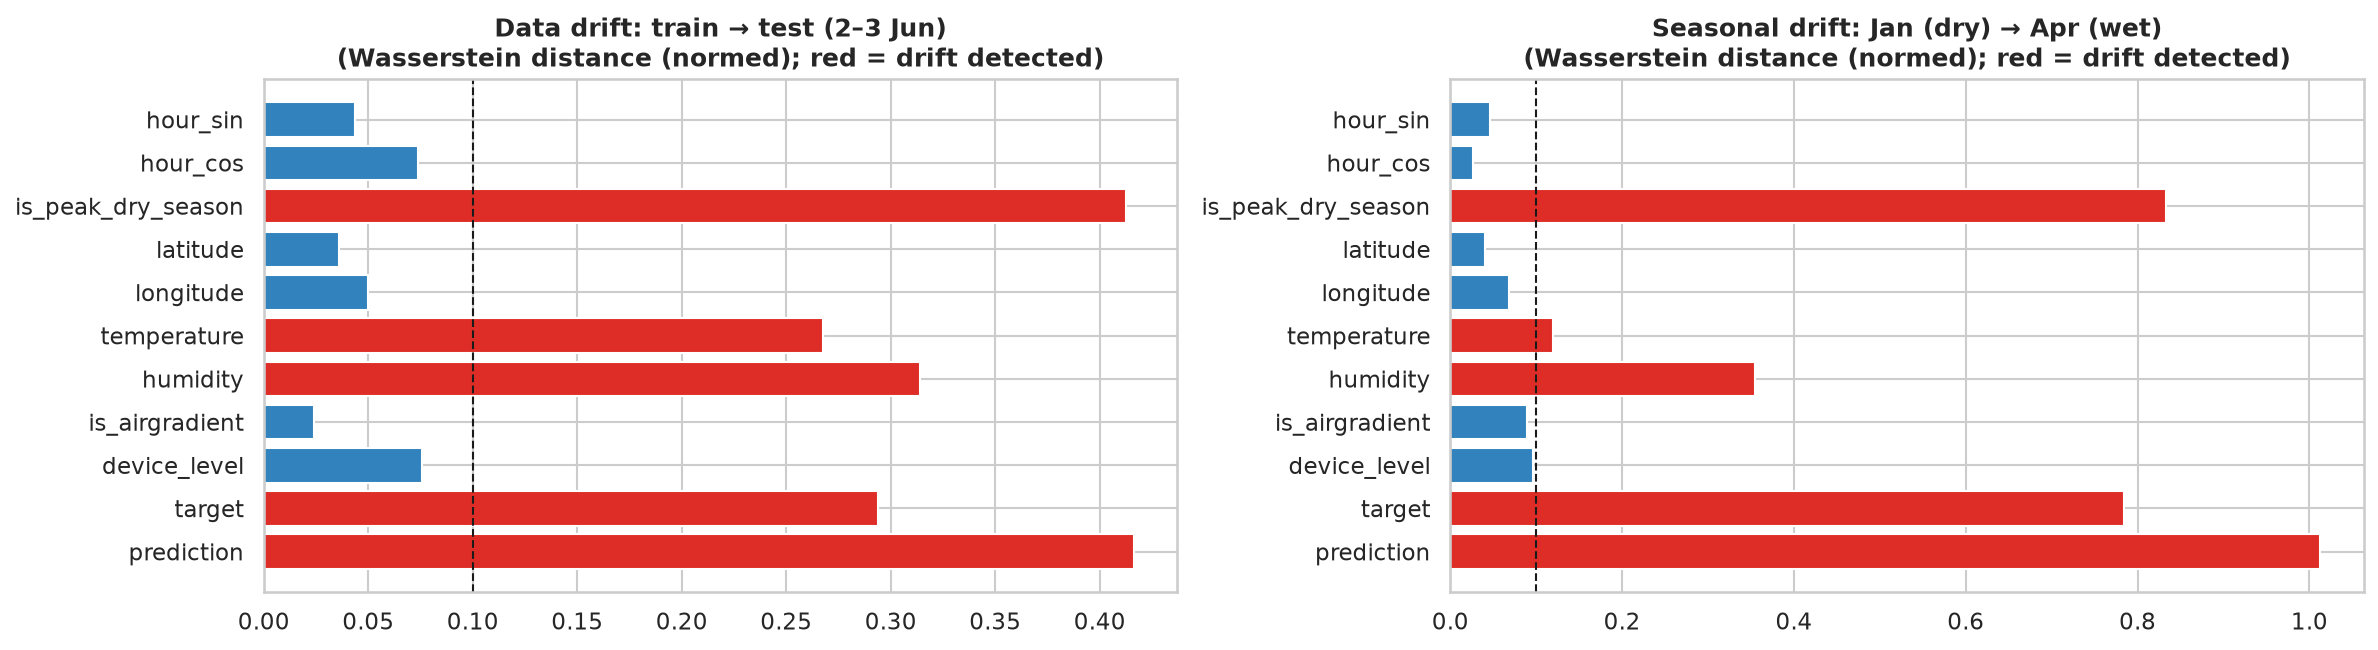
\includegraphics[width=\textwidth]{06a_evidently_drift.png}
\caption{Evidently drift scores; red bars exceed the drift threshold.}
\end{figure}

Five of eleven columns drift between training and test (below the 50\% dataset-drift threshold). The drifting columns are the weather variables, the season flag, the target and the predictions; time-of-day, location and device mix do not drift, so sensor coverage is stable and the drift is genuinely seasonal.

\begin{table}[H]
\centering\small
\caption{Model performance reported by Evidently (Z units).}
\label{tab:perf}
\begin{tabular}{lrrL{6.5cm}}
\toprule
Metric & Reference (train) & Current (test) & Interpretation \\
\midrule
RMSE & 0.517 & 0.704 & +36\%: generalisation gap on unseen hours \\
MAE & 0.351 & 0.432 & Smaller rise than RMSE: extra error is in spikes \\
Mean error & $-0.003$ & $-0.005$ & No systematic bias \\
$R^2$ & 0.733 & 0.222 & Much less variance explained out of sample \\
Max.\ absolute error & 5.94 & 5.89 & Worst miss $\approx 6\sigma \approx 168$\ugm{} in both \\
\bottomrule
\end{tabular}
\end{table}

\subsection{Monitoring policy}
In production, Evidently would run daily on newly labelled sensor data. Retraining is triggered when RMSE rises by more than about 20\% over the reference, when the mean error moves away from zero, or when the target drifts (for example, at the start of a dry season). Drift in time-of-day, location or device mix indicates a data-pipeline or coverage problem (sensors offline) that should be fixed rather than retrained on. The previous model version is kept so that a poorly performing retrained model can be rolled back. Three HTML reports are saved in \texttt{outputs/evidently/}.

% =================================================================
\section{Deployment on RunPod}
\subsection{Local debugging before deployment}
The full notebook was executed end-to-end locally before any cloud spending, as the brief requires. Table~\ref{tab:runtime} lists the stage timings logged by the pipeline (\texttt{outputs/logs/pipeline\_run.log}, \texttt{run\_summary\_local.json}); the whole run takes 251 s on four CPU cores without a GPU (Python 3.11, scikit-learn 1.9, XGBoost 3.2).

\begin{table}[H]
\centering\small
\caption{Local run: stage timings (seconds).}
\label{tab:runtime}
\begin{tabular}{lr@{\hspace{2.5em}}lr}
\toprule
Stage & Time & Stage & Time \\
\midrule
Load raw data & 0.1 & Tune Random Forest & 146.2 \\
Data preparation & 0.1 & Tune XGBoost & 20.0 \\
Hourly resampling & 0.7 & Stacking ensemble & 21.5 \\
Imputation & 4.5 & Forecasting & 0.2 \\
Tune Ridge / KNN / SVR & 2.0 / 3.4 / 10.3 & Evidently monitoring & 6.9 \\
\midrule
\multicolumn{3}{l}{\textbf{Total pipeline runtime}} & \textbf{250.7} \\
\bottomrule
\end{tabular}
\end{table}

\subsection{RunPod configuration and procedure}
RunPod is a pay-as-you-go GPU cloud; the budget for this stage is \$5.
\begin{enumerate}
\item \textbf{Service and Pod.} A \emph{Pod} (dedicated GPU instance for development and testing) on the Community Cloud, on-demand pricing.
\item \textbf{GPU.} An affordable, available GPU well under \$2/h (e.g.\ RTX A4000, RTX 3090 or RTX 4090, about \$0.2--0.7/h), checked in the Pod Summary and Pricing Summary before deploying; 20\,GB container disk and 20\,GB volume.
\item \textbf{Template.} RunPod PyTorch 2.x with Jupyter Lab.
\item \textbf{Import.} Clone the repository (code, data, shapefiles) and \texttt{pip install -r deployment/requirements.txt}.
\item \textbf{Run.} \texttt{bash deployment/run\_on\_runpod.sh} records \texttt{nvidia-smi}, the pod ID and the Python version, executes the notebook headless, and writes the executed notebook, \texttt{pipeline\_run.log} and \texttt{run\_summary\_runpod.json} (environment, GPU, stage timings, metrics, best model). XGBoost uses CUDA automatically.
\item \textbf{Shut down.} Download \texttt{outputs/} and \texttt{models/}, then stop and terminate the pod. Expected cost: about 15 minutes at \$0.4/h $\approx$ \$0.10 plus storage.
\end{enumerate}
If Evidently fails on the pod, the pipeline logs a warning and continues.

\begin{todobox}
\textbf{RunPod evidence --- to be completed after the run.} Insert: (1) the Pod Summary and Pricing Summary screenshots; (2) GPU name, hourly price and pod ID from \texttt{outputs/logs/runpod\_environment.txt}; (3) total runtime and stage timings from \texttt{run\_summary\_runpod.json}; (4) the best-model metrics printed on the pod (they should match Table~\ref{tab:results}); (5) a screenshot of the pod's \emph{Logs} tab and the billing page.
% Example once screenshots are saved in report/img/:
% \begin{figure}[H]\centering\includegraphics[width=0.9\textwidth]{img/runpod_pod_summary.png}\caption{RunPod pod summary and pricing.}\end{figure}
\end{todobox}

% =================================================================
\section{Limitations and future work}
\begin{itemize}
\item \textbf{Very short history.} Only seven days in three windows were available, so weekday effects, long-term trends and seasonal transitions cannot be learned or validated. Pulling months of continuous data from the AirQo API is the most valuable improvement.
\item \textbf{Climatological weather at forecast time.} August forecasts use June hour-of-day weather, so daily forecasts barely vary. Feeding numerical weather forecasts (e.g.\ UNMA or Open-Meteo) would add day-to-day skill.
\item \textbf{Spikes are under-predicted.} A dedicated nowcasting model with lag features, quantile regression for upper percentiles, or an exceedance classifier would improve early warnings.
\item \textbf{Season assumption.} August is coded like June (non-peak). If August is dustier, the model will under-predict; target-drift monitoring on real August data would reveal this.
\item \textbf{Operationalisation.} Automate the Evidently checks, retraining triggers, model versioning and rollback, and serve the model behind an endpoint.
\end{itemize}

% =================================================================
\section{Conclusion}
We delivered a reproducible, deployable PM2.5 pipeline for AirQo data. Careful auditing exposed that the data covers only three short windows, which led to gap-aware cleaning (short-gap interpolation, spatial weather imputation, no fabricated long-gap labels), a complete hourly grid, a chronological hold-out and blocked cross-validation. Kampala's air is mostly \emph{Moderate} to \emph{Unhealthy for Sensitive Groups}, with \emph{Unhealthy} episodes in the peak dry season, clear morning and evening peaks, and higher concentrations in cool, humid hours. XGBoost was the best of five tuned models and a stacking ensemble (RMSE 20.0\ugm, $R^2=0.22$, 71\% AQI accuracy) and was saved with everything needed to forecast in \ugm. Forecasts for August 2026 are mostly \emph{Moderate}, with central Kampala sites reaching USG levels at the morning peak. Evidently monitoring confirmed seasonal drift and quantified the generalisation gap, and the pipeline is packaged to run on a low-cost RunPod GPU pod.

% =================================================================
\begin{thebibliography}{9}
\bibitem{adong2022}
P.~Adong, E.~Bainomugisha, D.~Okure, and R.~Sserunjogi.
\newblock Applying machine learning for large scale field calibration of low-cost PM2.5 and PM10 air pollution sensors.
\newblock \emph{Applied AI Letters}, 3(3):e76, 2022.

\bibitem{barkjohn2021}
K.~K. Barkjohn, B.~Gantt, and A.~L. Clements.
\newblock Development and application of a United States-wide correction for PM2.5 data collected with the PurpleAir sensor.
\newblock \emph{Atmospheric Measurement Techniques}, 14(6):4617--4637, 2021.

\bibitem{junninen2004}
H.~Junninen, H.~Niska, K.~Tuppurainen, J.~Ruuskanen, and M.~Kolehmainen.
\newblock Methods for imputation of missing values in air quality data sets.
\newblock \emph{Atmospheric Environment}, 38(18):2895--2907, 2004.

\bibitem{okure2022}
D.~Okure, J.~Ssematimba, R.~Sserunjogi, N.~L. Gracia, M.~E. Soppelsa, and E.~Bainomugisha.
\newblock Characterization of ambient air quality in selected urban areas in Uganda using low-cost sensing and measurement technologies.
\newblock \emph{Environmental Science \& Technology}, 56(6):3324--3339, 2022.

\bibitem{roberts2017}
D.~R. Roberts, V.~Bahn, S.~Ciuti, M.~S. Boyce, J.~Elith, G.~Guillera-Arroita, et~al.
\newblock Cross-validation strategies for data with temporal, spatial, hierarchical, or phylogenetic structure.
\newblock \emph{Ecography}, 40(8):913--929, 2017.

\bibitem{who2021}
World Health Organization.
\newblock \emph{WHO Global Air Quality Guidelines: Particulate Matter (PM2.5 and PM10), Ozone, Nitrogen Dioxide, Sulfur Dioxide and Carbon Monoxide}.
\newblock WHO, Geneva, 2021.

\bibitem{evidently}
Evidently AI.
\newblock Evidently documentation: data drift and regression presets (v0.7).
\newblock \url{https://docs.evidentlyai.com}, 2026.
\end{thebibliography}

\end{document}
